
\documentclass[a4paper,12pt, english]{article} 

% Packages:

\usepackage{graphicx,xcolor} 
\usepackage{subfigure} 

\usepackage{amssymb}
\usepackage{amsmath}

\usepackage{float}
\usepackage[exponent-product=\cdot, per-mode=symbol]{siunitx} 
\usepackage[notrig]{physics} 
\usepackage{enumitem,lastpage,parskip} 
%\usepackage[hidelinks]{hyperref}
\usepackage{listings} 
\usepackage{cprotect} 
%\allowdisplaybreaks

\usepackage[utf8]{inputenc}
\usepackage[T1]{fontenc}
\usepackage{appendix}
\usepackage[colorlinks,linkcolor=blue]{hyperref}

\usepackage{booktabs}
\usepackage{minted}
\usepackage{comment}
\usepackage{url}
\usepackage{fancyhdr}
\usepackage[width=.9\textwidth]{caption}


%\usepackage{subcaption}
%\usepackage[pass]{geometry}

%Plot path
\graphicspath{ {./VelocityDistr/}}

%Bibliography stuff
\usepackage[
            backend=biber,
            citestyle=numeric,
            bibstyle=authoryear,
            sorting=none,
            ]{biblatex}
\usepackage[nottoc,numbib]{tocbibind}
\usepackage{emptypage}
\makeatletter
\input{numeric.bbx}
\makeatother

\addbibresource{bibliography.bib}
\AtEveryBibitem{\clearfield{isbn}}
\AtEveryBibitem{\clearfield{note}} 
\AtEveryBibitem{\clearfield{url}}
\AtEveryBibitem{\clearfield{doi}}
\AtEveryBibitem{\clearfield{issn}}
\AtEveryBibitem{\clearfield{month}}
\AtEveryBibitem{\clearfield{eprint}}
\DeclareNameAlias{author}{family-given}

% CODE ENVIRONMENT
\definecolor{mygreen}{rgb}{0,0.6,0} \definecolor{mygray}{rgb}{0.5,0.5,0.5} \definecolor{mymauve}{rgb}{0.58,0,0.82}
\lstset{basicstyle=\footnotesize, breakatwhitespace=false, breaklines=true, commentstyle=\color{mygreen}, extendedchars=true, frame=single, keepspaces=true, keywordstyle=\color{blue}, language=Python, numbers=left,                    numbersep=5pt, numberstyle=\tiny\color{mygray},  rulecolor=\color{black}, showspaces=false, showstringspaces=false, showtabs=false, stringstyle=\color{mymauve}, tabsize=3, title=\lstname, captionpos=b}


%Title, author(s) and date
\title{The Fate of the Solar System after Milky Way and Andromeda Merger}
\author{Alberto Brentegani, Davey Plugers, Zhen Xiang}
\date{13 December 2020}

% SET HEADER/FOOTER
\pagestyle{fancy}
\fancyhf{}
\fancyhead[R]{\thepage}  
\fancyhead[C]{\nouppercase{\leftmark}}  
\fancyhead[L]{\nouppercase{Group E}}  
\fancyheadoffset[R,L]{1cm}  
\renewcommand{\headrulewidth}{0.5pt}  

%defining caption for equation
\DeclareCaptionType{equ}[][]
%\captionsetup[equ]{labelformat=empty}

\begin{document}

%used to restore the default article layout after including the geometry package with the pass argument
%\restoregeometry

\begin{titlepage}
\makeatletter
\begin{center}

\vspace*{-1in}
\begin{figure}[htb]
    \centering
    
\includegraphics[width=8cm]{lu_logo.png}
\end{figure}

\vspace{-25pt}
\rule{125mm}{0.1mm} \\
\vspace{5pt}
\begin{Large}
    \textsc{Faculty of Science}\\
\end{Large}
\vspace{5pt}
\textit{Course of:}\\

\begin{Large}
    \textsc{Simulation and Modeling in Astrophysics}\\
\end{Large}
\vspace{30pt}

\begin{LARGE}
    \textbf{Group E Project Report:} \\
    \textbf{\@title} \\
\end{LARGE}
\vfill

\begin{normalsize}
	\begin{flushleft}
	  \textit{Date:} \hfill \textit{Students:}\\
	  \vspace{1pt}
	  \@date \hfill Alberto Brentegani\\
	  \hfill Davey Plugers\\
	  \hfill Zhen Xiang\\
	  \vspace{10pt}
	\end{flushleft}
\end{normalsize}
\vspace{20pt}

\rule{125mm}{0.1mm} \\
\vspace{5pt}
\scshape{\large{Academic Year 2020/2021}} \\

\end{center}
\makeatother
\end{titlepage}

%new layout for the text (if using geometry package)
%\newgeometry{
%    textheight=9in,
%    textwidth=6.5in,
%    top=1in,
%   headheight=14pt,
%    headsep=25pt,
%    footskip=30pt
%  }

%abstract
\begin{abstract}
The future merger between the Milky Way (MW) and Andromeda (M31) galaxy is a matter of great interest within the astrophysical community, given that it involves our host Galaxy, and in the past has been studied in several works, most notably by \textcite{Cox_2008}, using simulations and observational constraints.% In this work we will follow the simulation approach, with the help of the AMUSE framework, adding the Solar System into the MW-M31 system. Our goal is to find out what will be the fate of our own System after the merger event. Several scenarios are possible: it could remain bound to the new-formed galaxy, at a smaller or larger radial position compared to the present one, or it could be ejected into the intergalactic space. Taking into account a wide range of initial conditions (such as the M31 velocity vector, the galactic coordinates of the Solar System \iffalse and, if enough time is available, the presence of the Intergalactic Medium\fi) and using detailed galaxy models, we aim to find out the probability of these scenarios.
In this work we will follow the simulation approach, with the help of the AMUSE framework, adding the Solar System into the MW-M31 system. Our goals are to analyse the separation between the galaxies and the fate of our Solar System after the merger for different tangential and radial velocity components of the M31 galaxy. These simulations are done by with and without the presence of the IGM. For the non-IGM run, the result shows that the greater the velocity components, the later the first encounter will take place. By comparison, the IGM plays a major role in the merger process exerting friction on both galaxies and speeding up the merger process. Eventually, after the merger has completed, the Solar System is most likely be further away in the newly formed galaxy.\par
All code is publicly available on our \href{https://github.com/boson112358/sma-group-e-project}{GitHub repository}.
\end{abstract}

\newpage

\tableofcontents 

\newpage 

\section{Introduction}
\label{introduction}
Within the Local Group a macroscopic event is set to take place in the future: given that the Andromeda Galaxy is moving towards the Milky Way, the two galaxies are likely to experience a collision and a subsequent merger event in \(\approx 5\: Gyr\) (see \textcite{Cox_2008}, \textcite{van_der_Marel_2019} and \textcite{Schiavi_2019}). This immediately raises a question: at the end of such an event, what will happen to the Solar System? To get an answer our research will focus on simulating such a collision and merger using the AMUSE software (see \textcite{Portegies_Zwart_McMillan_2018}, \textcite{Portegies_Zwart_2013}, \textcite{Pelupessy_2013} and \textcite{Portegies_Zwart_2009}), with the goal to unravel the fate of the Solar System.\par
\smallskip
In our simulations we take into account the effect of both the Intergalactic Medium (IGM) and the M31 starting dynamical conditions on the merger event.\par
\smallskip

\subsection{Our Goals}
\label{goals}
During the merger event, we will focus on the motion of the Solar System within the MW-M31 frame. Our goals for this project are: 
\begin{itemize}
    \item to determine how the starting conditions of the simulation, as relative velocity and the presence of the IGM, affect the dynamical evolution of the merger;
    \item to infer the average position of the Solar System in the newly formed galaxy after the merger.
\end{itemize}
\par\smallskip

\subsection{Outline of the Report}
\label{outline}
In Section \ref{methods} we present the AMUSE framework and the modules we used to set up our simulations, namely \texttt{GalactICs}, \texttt{Gadget2} and \texttt{Fi}. We further describe the implementation of a leapfrog algorithm for the integration of the Solar System position.\par
\smallskip
In Section \ref{initial-conditions} we present the initial conditions of our MW, M31 and IGM models, as well as the initial relative displacement of the galaxies. Furthermore we describe how we add the Solar System to the MW model. \par
\smallskip
In Section \ref{results} we first analyse our galaxy models, to determine their accuracy and stability. Then we show the results of several merger simulations with different starting velocities for M31 and with the IGM. Furthermore, we analyse the distance distribution of the Solar System tracker particles.\par
\smallskip
In Section \ref{conclusions} we summarise the steps we took to run our simulations and we draw out our conclusions. We also present possible future developments.\par
\newpage

\section{Methods}
\label{methods}
The simulations are run through the implementation of two hydrodynamics modules within the AMUSE framework, \texttt{Gadget2} and \texttt{Fi}. Even though we finally opted to use only \texttt{Gadget2} for all the simulations, both solvers are implemented in our code to evolve the galaxy models, which are generated through the \texttt{GalactICs} module, specifically with the \texttt{new\_galactics\_model} function.\par
\smallskip
The Solar System will be indirectly tracked by defining a region around its current position in the galactic plane and monitoring the dynamical evolution of the tracker stars generated in this region. In order to do so we developed a simple leapfrog algorithm which evolve the position of the stars given the MW gravity potential. Our initial strategy was to use \texttt{Gadget2} for testing and \texttt{Fi} for the final runs, however \texttt{Fi} turned out too slow for the amount of simulations we ran so we decided to use only \texttt{Gadget2}.\par
\smallskip

\subsection{AMUSE}
\label{amuse}
The entirety of our work, from modelling the galaxies to running the simulations, is done within the Astrophysical Multipurpose Software Environment (AMUSE) framework (see \textcite{Portegies_Zwart_McMillan_2018}, \textcite{Portegies_Zwart_2013}, \textcite{Pelupessy_2013} and \textcite{Portegies_Zwart_2009}). The advantage of this approach is that AMUSE allows us to combine different gravitational and hydrodynamical solvers together with the model generator, thus we are able to operate a wide range of simulations without the need to completely rewrite our code.\par
\smallskip

\subsection{The GalactICs Module}
\label{galactics}
The first module we use is \texttt{GalactICs}, originally developed by \textcite{Kuijken_1995} (further versions are presented in \textcite{Widrow_2005} and \textcite{Widrow_2008}). This module sets up self-consistent, axisymmetric disk-bulge-halo galaxy models, particularly featuring a finite extent, making them suitable for N-body simulation. Moreover the models are generated to fit observational data, such as rotation curves (see Section \ref{model-analysis}), making this module a very suitable choice to reproduce real galaxies, as the MW and M31.\par
\smallskip

\subsection{The Gadget2 Module}
\label{gadget2}
The second module we use is \texttt{Gadget2}, presented in \textcite{Springel_2005} (see also \textcite{Springel_2001} and \textcite{Durier_2012}). This simulation code is a parallel TreeSPH code and computes gravitational forces with a hierarchical tree algorithm. When simulating an isolated system, such as the MW-M31 system, it follows the evolution of a self-gravitating collisionless N-body system, further allowing gas dynamics to be optionally included. Owing to the fact that this code is a parallel tree code, it is able to quickly run our simulations.\par
\smallskip
Unfortunately this module is not well suited to be used with the \texttt{bridge} feature of AMUSE, which allows to combine different solvers, in order to solve dynamic problems due to the lack of the implementation of the \texttt{get\_gravity\_} \texttt{at\_point} method. This method outputs the gravitational acceleration that an object would experience in a certain position, so it is of fundamental importance to run gravitational nbody simulations. To solve this issue we implemented this method in a wrapper class of the \texttt{Gadget2} module, called \texttt{Gadget2Gravity}.\par
\smallskip
However after this new implementation we finally opted to include all the particle objects in our simulations (galaxies, Solar System trackers and IGM) within a single instance of \texttt{Gadget2}, to increase the speed of the code and to make it more straightforward. The total mass of the Solar System trackers (more on this in Section \ref{solar-system}), \(M = 10^3\: M_{\odot}\), is negligible compared to the total mass of the MW \(M_t = 10^{12} M_{\odot}\), so the addition of these particles to the Galaxy model does not have a disruptive influence on the overall stability.\par
\smallskip

\subsection{The Fi Module}
\label{fi}
The third module we use is \texttt{Fi} (see \textcite{Hernquist_1989}, \textcite{Gerritsen_1999}, \textcite{Pelupessy_2004} and \textcite{Pelupessy_2005}). It is a parallel TreeSPH code for galaxy simulations, thus suited to evolve the MW-M31 system. Compared to \texttt{Gadget2}, given the same galactic model, it has a larger run time. The \texttt{get\_gravity\_at\_point} method is fully implemented in this module. Due to the considerable time difference, we decided to use \texttt{Gadget2} for the final merger simulations.\par
\smallskip

\subsection{The Leapfrog Algorithm}
\label{leapfrog}
While not an AMUSE module, this algorithm is commonly used in astrophysics and provides much greater accuracy as oppose to direct integration. The algorithm works by adjusting the velocity and position at separate equidistant timesteps. It is a surprisingly simple yet powerful differential equation solver. In the code this is done by calling the \texttt{get\_gravity\_at\_point} method to get the acceleration for each one of the particles. This can then be used to adjust the velocity which determines the next particle position.\par
\smallskip
Even though the algorithm is written in a slower programming language (Python), compared to the underlying \texttt{Fi} language, this can still save time since it disregards the Solar System gravitational contribution as the main solver is handling the MW-M31 system, while keeping a lower complexity. This fact is shown by Equations \ref{eqn:complexity1} and \ref{eqn:complexity2}, where in the second equation $N_{Sol}$ is highlighted in red to denote the slower programming language.
\begin{align}
    \mathcal{O}(combined) &= (N_{gal}+N_{Sol})^2 \nonumber \\ 
    &\propto N_{gal}^2 + N_{gal}N_{Sol} + N_{Sol}^2 \label{eqn:complexity1}
\end{align}
\begin{align}
    \mathcal{O}(divided) &= N_{gal}^2 +  \mathcal{O}(\texttt{get\_gravity\_at\_point})\textcolor{red}{N_{Sol}} \nonumber \\
    &\propto N_{gal}^2 + ln(N_{gal})\textcolor{red}{N_{Sol}} \label{eqn:complexity2}
\end{align}\par
\smallskip
The \texttt{get\_gravity\_at\_point} method can be applied to all the Solar System particle positions to get their acceleration. We can further use a leapfrog integration to solve the second order differential equation defined by:
\begin{equation}
    \frac{d^2x}{dt^2} = A(x)
\end{equation}
This method is a second order differential equation method for periodic motion. Allowing for good accuracy for very little calculation for the Solar System particles. This is done by calculating $\frac{dx}{dt}$ and x at intermittent timesteps.\par
\smallskip
We start by defining a constant timestep and calculating the kick-velocity  $\vec{v}_{\frac{1}{2}}$. Once this has been calculated, the kick-velocity can be used to find a new position. This new position is then used to get the acceleration at that point which then calculates the new velocity. This process then repeats itself for as many timesteps as needed.
\begin{equation}
\begin{gathered}
    A(\vec{r}_i) = \verb+get_gravity_at_point+(\vec{r}_i) \\
    \vec{v}_{\frac{1}{2}} = \vec{v}_0 + A(\vec{r}_0)\frac{\Delta T}{2}\\
    \vec{r}_{i+1} = \vec{r}_i + \vec{v}_{i+\frac{1}{2}}\Delta T \\
    \vec{v}_{i+\frac{1}{2}} = \vec{v}_{i-\frac{1}{2}} + A(\vec{r}_i)\Delta T
\end{gathered}
\end{equation}\par
\smallskip
This code can then be run alongside the gravity solver to track the evolution of the Solar System throughout the merger.\par
\newpage

\section{Initial Conditions}
\label{initial-conditions}
To achieve our goals we need to consider the Solar System as a member of the MW and our Galaxy as a member of the Local Group. These two galaxies are its two most massive members that, according to recent simulations (see \textcite{Cox_2008}, \textcite{van_der_Marel_2019} and \textcite{Schiavi_2019}) and observational measurements (see \textcite{van_der_Marel_2012b}), are likely to experience a merger event in \(\approx 5\: Gyr\).\par
\smallskip
In order to simulate the merger, we consider the MW-M31 system to be isolated, without any influence from the other members of the Local Group (even though \textcite{van_der_Marel_2012b} suggest that the M33 galaxy will play an active role in the merger). Furthermore, we need to carefully model both the MW and M31, set their relative displacement and add the Solar System on top of the Galaxy. In this Section we give an overview of the initial conditions adopted into our merger model.\par
\smallskip

\subsection{Milky Way and Andromeda Models}
\label{mw-m31-models}
The \texttt{new\_galactics\_model} function of the \texttt{GalactICs} module takes several parameters as arguments. To determine these parameters we refer to \textcite{Widrow_2005}, \textcite{Widrow_2008} and the Master thesis from \textcite{Withagen_2019}, where both galaxies are modelled with the same module. In order to get representative models we choose the values taking an additional constraint into account: the rotation curves given by our models need to reproduce the observed rotation curves (see Sections \ref{model-analysis} and \ref{resutls}).\par
\smallskip
First we set the number of particles of the models, according to \textcite{Withagen_2019}, 70,000 is a right choice to build a realistic model. Thus we follow this approach and use these number of particles respectively for the halo, the disk and the bulge: \(n_{h} =\) 40,000; \(n_{d} =\) 20,000 and \(n_{b} =\) 10,000. This 4:2:1 proportion between the galaxy components comes from the default values of the module. Then the main galaxy macroscopic components (bulge, disk and halo) are generated by the code using the parameters in Table \ref{gal-param}. It is worth to stress the fact that both halo and bulge mass are not free parameters, they depend on disk mass and other parameters. The velocity, density and radius' cut-off of the halo are defined respectively by the \(\sigma_{h}\), \(a_{h}\) and \(\alpha_{h}\) parameters. The \(R_{d}\), \(R_{out}\), \(\delta R_{out}\) and \(h_{d}\) parameters define the geometry of the disk, while \(M_{d}\) defines its mass. The density and cut-off of the bulge are defined by \(a_{b}\) and \(\alpha_{b}\).\par

\begin{table}[]
\begin{tabular}{l|l|l|l|l}
Parameter          & Description                       & MW      & M31    & Unit               \\ \hline
\(\sigma_{h}\)     & Halo characteristic velocity      & 249.6   & 337.1  & km s\(^{-1}\)      \\
\(a_{h}\)          & Halo scale length                 & 12.96   & 12.94  & kpc                \\
\(\alpha_{h}\)      & Halo cut-off parameter            & 0.83    & 0.75   & -                  \\
\(M_{d}\)          & Disk mass                         & 45.8078 & 77.822 & \(10^9 M_{\odot}\) \\
\(R_{d}\)          & Disk scale length                 & 2.806   & 5.577  & kpc                \\
\(R_{out}\)        & Disk truncation radius            & 30      & 30     & kpc                \\
\(\delta R_{out}\) & Sharpness of disk truncation           & 1.0     & 1.0    & -                  \\
\(h_{d}\)          & Disk scale height                 & 0.409   & 0.3    & kpc                \\
\(\sigma_{R0}\)    & Radial velocity disperion at GC   & 70      & 80     & km s\(^{-1}\)      \\
\(R_{\sigma}\)     & Scale length of radial dispersion & 2.806   & 5.577  & kpc                \\
\(a_{b}\)          & Bulge scale length                & 0.788   & 1.826  & kpc                \\
\(\alpha_{b}\)     & Bulge cut-off parameter           & 0.787   & 0.929  & -                  \\ \hline 
\end{tabular}
\caption{\texttt{GalactICs} parameter for MW and M31 galaxies, see \textcite{Widrow_2005} and \textcite{Withagen_2019}.}
\label{gal-param}
\end{table}
\smallskip
Unfortunately when using the physical parameters in addition to the particle numbers to generate the models, we encountered a bug in \texttt{GalactICs}: a division by 0 within the \texttt{quantities} module. This bug is still unsolved so we opted to generate models that are not strictly representative of the MW and M31, but they are still a good approximation. The only parameter that did not make the model generation script crash is \(M_{d}\), so this is the only parameter we used, together with the particle numbers.\par
\smallskip
Our code generates the galaxy models taking the following assumptions:
\begin{itemize}
    \item The galaxies are axisymmetric with respect to the z-axis. This is a direct consequence of the \texttt{GalactICs} module, since it generates axisymmetric models. Although the majority of galaxies present non-axixymmetric features, such as bars or spiral arms, these could cause instabilities in the N-body simulations.
    \item The galaxies consist only of three main components: bulge, disk and dark matter halo. This is another pre-requisite for using \texttt{GalactICs}, since it takes arguments only for these macroscopic features. Consequently we are not considering globular clusters and stellar halos.
    \item The galaxies feature an isotropic velocity distribution.
    \item The galaxies are modelled only with collisionless particles, not taking into account the gas component of the disks.
    \item The galaxies do not feature a central SMBH. This feature is present in the original \texttt{GalactICs} code, but it has not been implemented within AMUSE yet.
\end{itemize}\par
\smallskip

\subsection{Andromeda Displacement}
\label{m31-displacement}
The evolution of the MW-M31 merger is highly sensitive to the magnitude of the transverse velocity of M31. For the value of this velocity vector, no general agreement has been reached, as in the past several values have been proposed (see \textcite{van_der_Marel_2012b}, \textcite{Salomon_2016} and \textcite{van_der_Marel_2019}) in a range that spans from \(\approx 10\: km/s\) to \(\approx 10^2\: km/s\). Given this wide uncertainty our simulations are run taking into consideration several values from the range of possible M31 transverse velocity vectors.\par
\smallskip
After setting the galactic parameters of the Milky Way and Andromeda, we need to set up the MW-M31 system. Following the approach of \textcite{van_der_Marel_2008}, we adopt Cartesian coordinates, with the centre of the Milky Way as the origin, the x-axis pointing from the Solar System to the Galaxy centre, the y-axis corresponding to the direction of the rotation of the Solar System around the centre of the Galaxy, and the z-axis pointing perpendicularly to the Galaxy plane. For a more detailed derivation of the displacement of the MW-M31 system, refer to \textcite{Withagen_2019}.\par
\smallskip
Concerning the rotation of two galaxies, the spin axis of the Milky Way is not parallel to Andromeda, so we need to rotate Andromeda. We can rotate Andromeda using equation:
\begin{equation}
    \boldsymbol{r_{M31}} = \boldsymbol{R_{M31}r}
\end{equation}
with,
\begin{equation}
    \boldsymbol{R_{M31}} = \left(\begin{array}{ccc}
         0.7703 & 0.3244 & 0.5490 \\
         -0.6321 & 0.5017 & 0.5905 \\
         -0.0839 & -0.8019 & 0.5915
    \end{array}\right)
\end{equation}
and $ \boldsymbol{r_{M31}} $ and $ \boldsymbol{r} $ is the rotated and unrotated position \iffalse vector\fi of Andromeda. This rotation matrix is found through the inclination and ascension of the Andromeda galaxy, combined with the earth's relative orientation with respect to MW. The resulting matrix then gives a simple three-dimensional rotation on the unit sphere.\par
\smallskip
Now we can use position vector $ \boldsymbol{r_{M31}} $ to translate Andromeda to the correct coordinates:
\begin{equation}
    \boldsymbol{P} \equiv \left(-389.2,+612.7,+283.1\right) kpc
\end{equation}\par
\smallskip
Then we calculate the radial and transverse velocity components to M31. We first find the opposed unit vector of the position vector,
\begin{equation}
    \boldsymbol{-\hat{P}} = \frac{\boldsymbol{-P}}{|\boldsymbol{P}|} = \left(+0.4898,-0.7914,+0.3657\right)
\end{equation}\par
\smallskip
To get radial velocity component, we can multiply this vector with the observed radial velocity.
\begin{equation}
    \boldsymbol{v_{rad}} = \boldsymbol{-\hat{P}}117 km s^{-1}
\end{equation}\par
\smallskip
To obtain the transverse velocity component one can define an orthogonal vector $ \boldsymbol{A}$, 
\begin{equation}
    \boldsymbol{A} \equiv \left(x,y,1\right)
\end{equation}\par
\smallskip
This describes a plane of possible vectors which are all orthogonal to the radial component. However for convenience we choose y=1 to get a single vector out of this plane. The reasoning behind this is that we assume our result is not dependent on the exact orientation of the tangential vector. This vector $\boldsymbol{A} = \left(x,1,1\right)$ is perpendicular to vector $ \boldsymbol{P} $,
\begin{equation}
    \boldsymbol{-\hat{P}}\cdot\boldsymbol{A} = 0
\end{equation}\par
\smallskip
This gives us the value of x. Similarly, we can get the unit vector of $\boldsymbol{A}$ 
\begin{equation}
    \boldsymbol{\hat{A}} = \left(0.5236,0.6024,0.6024\right)
\end{equation}\par
\smallskip
Now we get the transverse velocity component $ \boldsymbol{v_{trans}} $
\begin{equation}
    \boldsymbol{v_{trans}} = 42 km s^{-1} \boldsymbol{\hat{A}}
\end{equation}\par
\smallskip
To simulate various starting velocities we introduced two tuning factors in the final radial and transverse velocity vectors: \(f_{r}\) and \(f_{t}\) respectively.\par
\smallskip

\subsection{Solar System}
\label{solar-system}
To simulate the Solar System there are different methods that can be used. One can add a particle to the gravity solver and look where it ends up. However, due to uncertainties and inaccuracies in position and velocity, this single particle approach will not give a good prediction.\par
\smallskip
A solution to this can be found by using statistics. By evolving many different particles at suitable locations, it is possible to get a statistical likelihood of certain outcomes for the Solar System. One such possibility is to use the distance between the Sun and the centre of the Galaxy as a fixed parameter and then generate a ring distribution of particles at this radius. Another possibility is to define the exact location of the solar system and then define a small area in which we can distribute particles.\par
\smallskip
The advantage of this second method is that it can give a much better prediction given the right initial conditions. On the other hand, the disadvantage of this approach is that its results can be much worse compared to the ring model in the case our starting values are not correct. For the time being we opt to use the position model, however later simulations might switch back to the ring model if we keep struggling to fix our galaxy models.\par
\smallskip
While adding these particles in the right position is a great starting point, we still need to make them evolve in time. One option is to just add them to the \texttt{Fi} solver that we are using, however this method has some major disadvantages.\par
\smallskip
First, if we want to distribute our mass properly across the galaxy, suddenly adding an enormous amount of stars in a certain point could destroy this balance, making the Galaxy model unstable. The simulations are run with 1000 tracker particles, so the the total mass is ($10^4$M$_{\odot}$). This value is many orders of magnitude smaller than the mass of a single galaxy particle ($\approx 10^7$ M$_{\odot}$) and than the total galaxy mass ($\approx 10^{12}$ M$_{\odot}$). If needed the mass of the tracker particles could even be set to zero since we are not interested in their gravitational effect on the MW-M31 system but how the system affects their position. \par
\smallskip

\subsection{Intergalactic Medium}
\label{Intergalactic Medium}
In the process of simulating the MW-M31 merger, we considered the addition of the Intergalactic Medium (IGM). Due to its presence, galaxies will be affected by friction during their motion.\par
\smallskip
Based on the above considerations, and following the approach of \textcite{Cox_2008}, we assume that the IGM of the Local Group is represented by a constant density distribution within a 1 Mpc side cube. In addition we assume the IGM to be made of only two components: dark matter and gas. We set the mass fractions of these components to be 20\% primordial gas and 80\% dark matter. The temperature of the gaseous component is assumed  to be $3\cdot10^5$ K. We further assume the total IGM mass to be equivalent to the total mass of the MW-M31 system, \(M = 2 \times 10^{12} M_{\odot}\), and the number of IGM particles to be equal to the total number of particles of the two galaxies: $2(n_h+n_d+n_b) = 70000$. Therefore, we generate the IGM model using the parameters in Table \ref{igm-param}.

\begin{table}[]
\begin{tabular}{l|l|l|l}
Parameter        & Description                         &Value             & Unit               
\\ \hline
\(N1\)           & Number of IGM dark matter particles &70000             & -  
\\
\(N2\)           & Number of IGM gas particles         &70000             & -   
\\
\(box\_side\)     & Side length of cube                 &1000             & kpc    
\\
\(\rho\)         & Density of IGM                      &770               & M$_{\odot}$kpc$^{-3}$
\\
\(u\)            & Gas internal energy                &$3.724\cdot10^9$  & m$^2$s$^{-2}$
\\
\hline 
\end{tabular}
\centering
\caption{Parameters for setting up IGM}
\label{igm-param}
\end{table}

\subsection{Model analysis}
\label{model-analysis}
When creating the galaxy model it is fundamental to make sure that all the particles have been generated accordingly to our initial conditions. To make sure the position is correct we plot the particle data set to see their spatial distribution on the x-y plane. However to check the velocity components we need to do some preliminary calculations. In our code the velocity of the particles is defined by three different components: $v_x, v_y$ and $v_z$. Our approach to the problem is to convert them into spherical velocity components: $v_{rad}, v_{ang}$ and $v_{tan}$, being respectively the radial, angular and tangential components. For each particle of the models, the radial unit vector is calculated along the distance vector between that particle and the centre of mass of the galaxy, the angular unit vector is defined to be on the x-y plane and the tangential velocity is defined such that it is perpendicular to the other two unit vectors.\par
\smallskip
First we redefine the position of each particle into a cartesian coordinate system with the origin in the centre of mass of the galaxy, which is done by taking the position $\vec{r}$ and subtracting the centre of mass position $\vec{r}_{CoM}$.
\begin{equation}
    \begin{pmatrix}
    x'\\y'\\z'
    \end{pmatrix}
    = 
    \begin{pmatrix}
    x\\y\\z
    \end{pmatrix}
    - 
    \begin{pmatrix}
    x_{CoM}\\y_{CoM}\\z_{CoM}
    \end{pmatrix}
\end{equation}\par
\smallskip
Once we have these x', y' and z' coordinates, these can be redefined into the spherical coordinates \(r\), \(\theta\) and \(\phi\):
\begin{equation}
\begin{gathered}
    r = \sqrt{x^{\prime2} + y^{\prime2} + z^{\prime2} }\\
    \theta = \arctan \left( \frac{\sqrt{x^{\prime2} + y^{\prime2}}}{z'} \right)\\ 
    \phi = \left\{ \begin{array}{ll}
             \arctan\left(\frac{y'}{x'}\right)\ \ \ \ \ \ \ \ \ \ \  x' < 0 \\
            \arctan\left(\frac{y'}{x'}\right) + \pi \ \ \ \ \ \  x' > 0 
        \end{array} \right.
\end{gathered}
\end{equation}\par
\smallskip
The different values for $\phi$ are due to the definition of the \(\arctan\) function. When defined like this we have $\theta \in [-\frac{\pi}{2}, \frac{\pi}{2}]$ and $\phi \in [-\frac{\pi}{2}, \frac{3\pi}{2}]$. With these values it is possible to define the local orthogonal vectors for our particle. 
\begin{equation}
\begin{gathered}
\hat{r} = \sin\theta\cos\phi \ \hat{x} + \sin\theta\sin\phi \ \hat{y} + \cos\theta \ \hat{z} \\
\hat{\theta} = \cos\theta\cos\phi \ \hat{x} + \cos\theta\sin\phi \ \hat{y} - \sin\theta \ \hat{z} \\
\hat{\phi} = -\sin\phi \ \hat{x} + \cos\phi \ \hat{y}
\end{gathered}
\end{equation}\par
\smallskip
However we can also get $\hat{r}$ by taking the redefined position vector and dividing it by its magnitude. Since we are going to plot these velocities in function of their distance $|\vec{r}-\vec{r}_{CoM}|$, this will be the preferred method.  
\begin{equation}
    \hat{r} = \frac{\vec{r}-\vec{r}_{CoM}}{|\vec{r}-\vec{r}_{CoM}|}
\end{equation}\par
\smallskip
Now we can solve for the three new velocity components by using the velocity of the particle and expressing it in the different orthogonal bases.
\begin{equation}
    v_x \ \hat{x} + v_y \ \hat{y} + v_z \ \hat{z} = \vec{v} = v_{rad} \ \hat{r} + v_{ang} \ \hat{\phi} + v_{tan} \ \hat{\theta}
\end{equation}\par
\smallskip
Taking the inner product with $\hat{x}, \hat{y}$ and $\hat{z}$ then gives three linear equations that can be solved to get the values for $v_{rad}, v_{ang}$ and $v_{tan}$.\par
\smallskip
It is important to note that if we are considering a galaxy particle whose rotation is not restricted to the x-y plane, we need to redefine the $\hat{\phi}$ which then will also change $\hat{\theta}$. This is because now $\hat{\phi}$ is defined to lie in the rotational plane such that its velocity component $v_{ang}$ is the speed at which it rotates around the galaxy. Then we plot the three spherical velocity components in function of their distance and check if they are correct.\par
\smallskip
Most of these components should average out to zero except for the angular velocity. A relevant aspect of this analysis is the variance of the velocities. Obviously not every particle should move with exactly 0 km/s for the tangential or radial component, however if this variance is too big the galaxy will be unstable and lose its structure.\par
\smallskip
After considering each velocity component individually, we then focus on the magnitude of the total velocity $\vec{v}$. This value in function of the distance from the centre of mass is important since this will give the rotation curve of the galaxies. If we plot this curve for our galaxy models we should get a profile similar to the observed curves, shown in Figures \ref{fig:obs-mw-curve} and \ref{fig:obs-m31-curve}. For a further discussion about the rotation curve see section \ref{Simulation Stability}\par
%%write about rotation curve, how we compute that and why it is useful. Maybe add a sample plot of m31 rotation curve
\begin{figure}[!h]
    \centering
    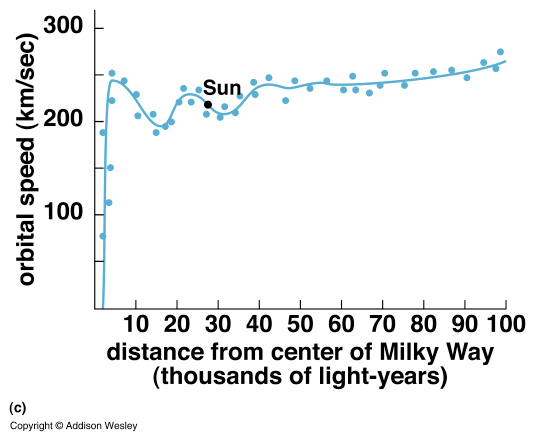
\includegraphics[width=0.55\linewidth]{Rotation_Curve.jpg}
    \caption{Observed MW rotation curve, taken from \textcite{Obennet_2017}.}
    \label{fig:obs-mw-curve}
\end{figure}

\begin{figure}[!h]
    \centering
    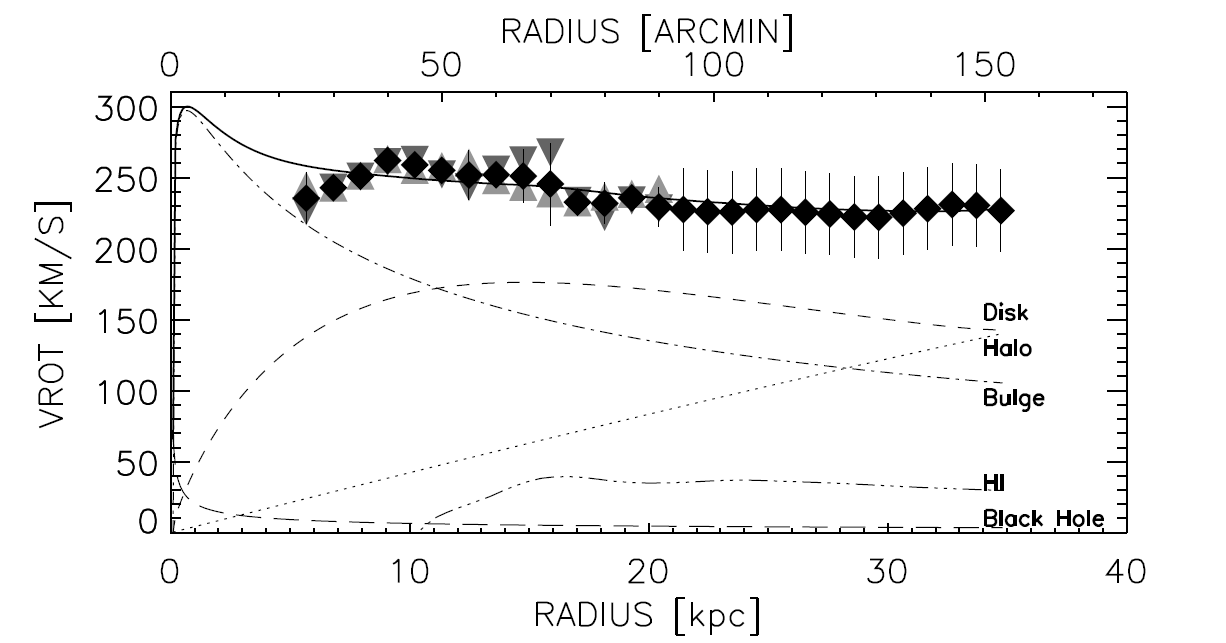
\includegraphics[width=0.7\linewidth]{observed_m31_rot_curve.png}
    \caption{Observed M31 rotation curve, taken from \textcite{Carignan_2006}.}
    \label{fig:obs-m31-curve}
\end{figure}

\begin{comment}
    These observed values can be compared with our rotation curves, shown in Figures \ref{fig:mw-rot-curve} and \ref{fig:m31-rot-curve}. After having corrected the velocity of the particles by a 0.15 factor, at small radii the simulated and observed curves appear to be very similar in shape. However at larger radii the simulated curves deviate substantially from the expected profiles. This discrepancy shows that our models are not a good approximation of the galaxies.\par

    \clearpage
    
    \section{Old Results}
    \label{resutls}
    In this Section we show the plots resulting from the galaxy model analysis described in Section \ref{model-analysis} as well as snapshots of our simulation, both of the MW and of the MW-M31 merger. As our models are not stable yet, all the velocities are plotted after multiplying the cartesian components of the velocity by a factor 0.15, in order to obtain values within the same order of magnitude of the observed ones. Furthermore in the simulations, in addition to the velocity correction, the total mass of the galaxies has been multiplied by a 0.001 factor.\par
    \smallskip
    In the panels of Figure \ref{fig:mw-m31-merger-evolution} is shown the instability of the galaxy models. In the panels of Figure \ref{fig:mw-evolution} we observe in more detail the instability of the MW galaxy model over relatively small timescales. Figures \ref{fig:mw-rot-curve} and \ref{fig:m31-rot-curve} show the simulated rotation curves. Figures \ref{fig:bulge-vel}, \ref{fig:disk-vel} and \ref{fig:halo-vel} show the velocity distributions of different Galaxy components.\par
    
    \begin{figure}[!ht]
    \centering
    \begin{minipage}{0.45\textwidth}
      \centering
    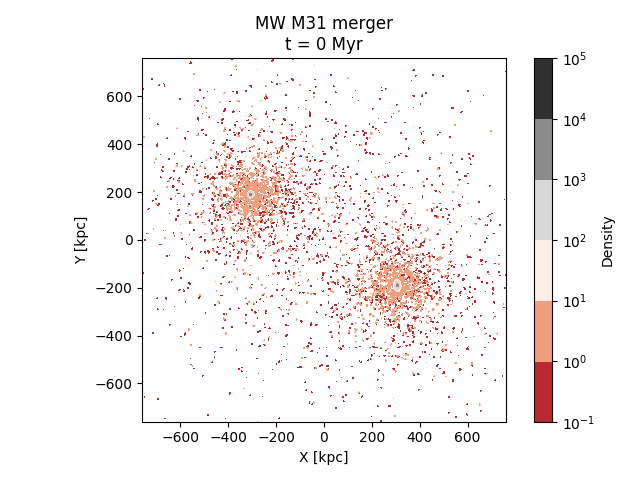
\includegraphics[width=1\textwidth]{simulations-plots/mw_m31_cmerger_0000.png}
    \end{minipage}
    \begin{minipage}{0.45\textwidth}
      \centering
    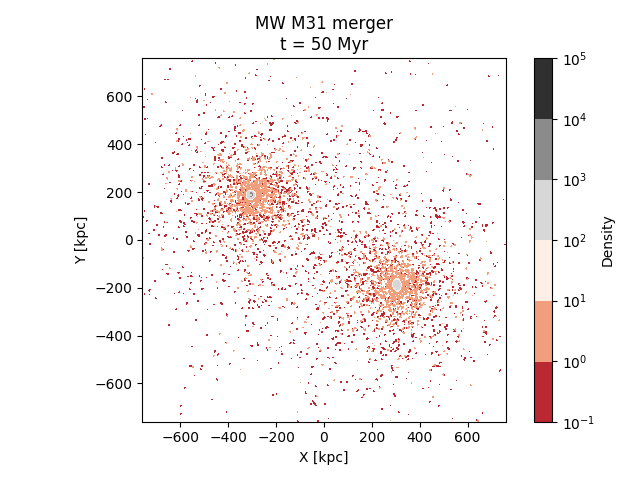
\includegraphics[width=1\textwidth]{simulations-plots/mw_m31_cmerger_0010.png}
    \end{minipage}
    \begin{minipage}{0.45\textwidth}
      \centering
    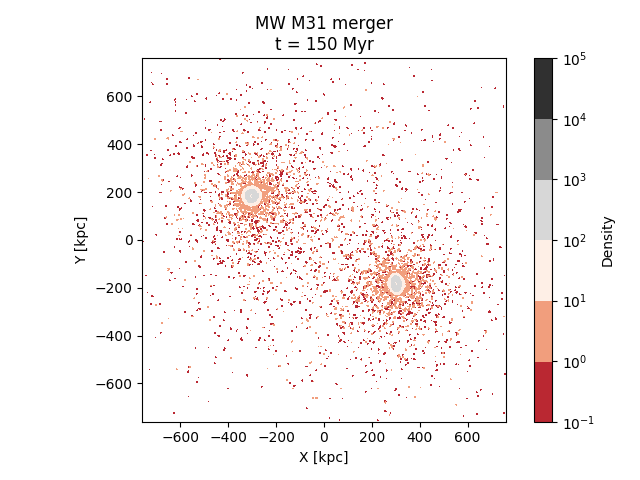
\includegraphics[width=1\textwidth]{simulations-plots/mw_m31_cmerger_0030.png}
    \end{minipage}
    \begin{minipage}{0.45\textwidth}
      \centering
    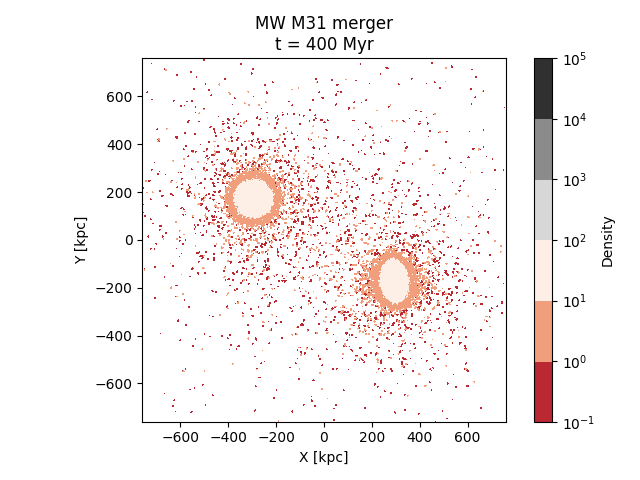
\includegraphics[width=1\textwidth]{simulations-plots/mw_m31_cmerger_0080.png}
    \end{minipage}
    \caption{Contour plot of the number density time evolution of the MW-M31 system, result of a simulation run with \texttt{Gadget2} with a timestep of 0.5 Myr. Note that before running the code the mass and the velocity of both galaxies were multiplied respectively by a 0.001 and a 0.15 factor. The x-y plane is assumed to be parallel to the MW galactic plane. From left to right, top to bottom the time of the simulation increases.} 
    \label{fig:mw-m31-merger-evolution}
    \end{figure}
    
    
    \begin{figure}
    \centering
    \begin{minipage}{0.45\textwidth}
      \centering
    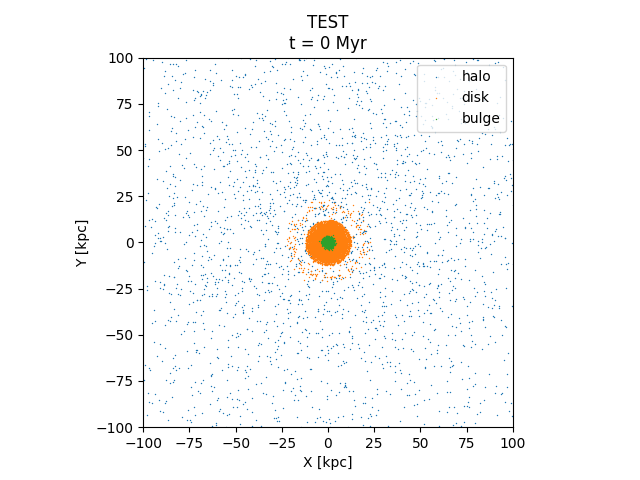
\includegraphics[width=1\textwidth]{simulations-plots/mw_testrun_0000.png}
    \end{minipage}
    \begin{minipage}{0.45\textwidth}
      \centering
    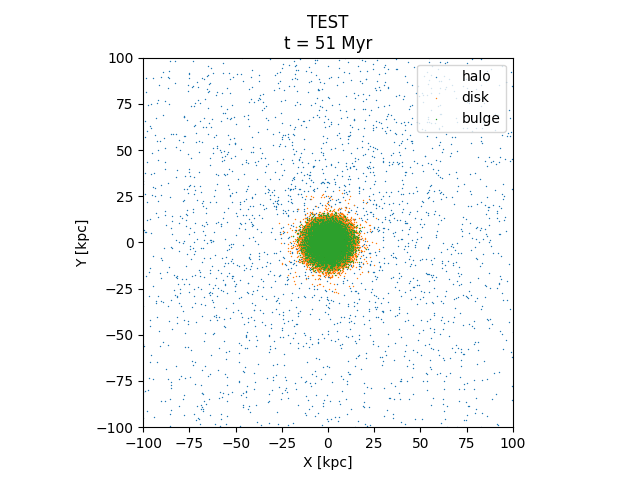
\includegraphics[width=1\textwidth]{simulations-plots/mw_testrun_0046.png}
    \end{minipage}
    \begin{minipage}{0.45\textwidth}
      \centering
    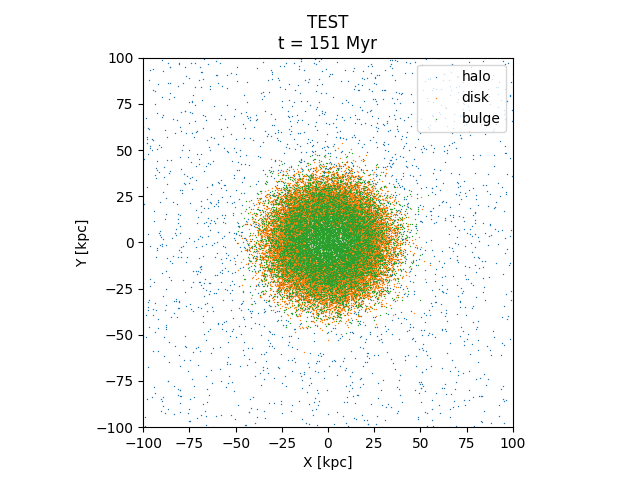
\includegraphics[width=1\textwidth]{simulations-plots/mw_testrun_0137.png}
    \end{minipage}
    \begin{minipage}{0.45\textwidth}
      \centering
    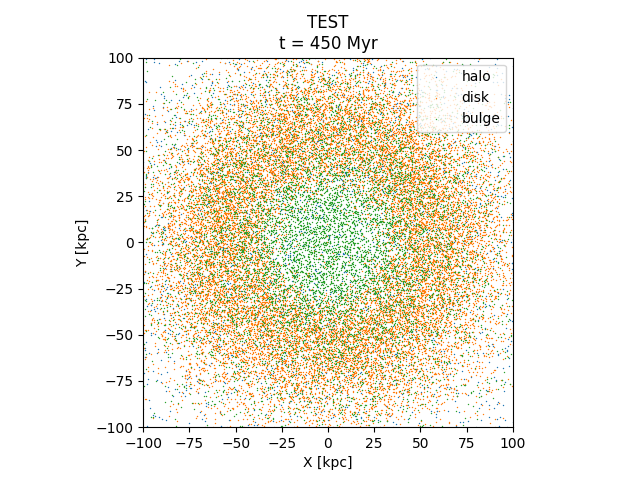
\includegraphics[width=1\textwidth]{simulations-plots/mw_testrun_0409.png}
    \end{minipage}
    \caption{Coordinate time evolution of the MW components, result of a simulation run with \texttt{Gadget2} with a timestep of 0.5 Myr. Note that before running the code the mass and the velocity were multiplied respectively by a 0.001 and a 0.15 factor. The x-y plane is assumed to be parallel to the MW galactic plane. From left to right, top to bottom the time of the simulation increases.} 
    \label{fig:mw-evolution}
    \end{figure}
    
    
    
    %Add some plots showing the variance of the radial and tang velocity/ add a plot for the angular/velocity profile, comment how we may need to change some stuff in the halo to get better resembling velocity profile and how we are looking for the parameter to change the velocity dispersion
    
    \clearpage
\end{comment}
\newpage

\section{Results}
\label{results}
In this section we demonstrate the stability of our galaxy models as well as the short term evolution of the Solar System tracker particles. Then the non-IGM simulations are analysed for different velocities by looking at the separation of the galaxies' centre of mass as a function of time. The same will be done for the IGM simulations with different values of tangential velocities for M31.\par
\smallskip

\subsection{Galaxy Model Stability}
\label{Simulation Stability}
Many of the early simulations suffered from bad initial conditions resulting in unstable galaxies and causing the models to be non-representative of their physical counterpart. Because we performed an accurate preliminary stability analysis.\par
\smallskip
To start we need to make sure the rotation curve of our galaxy created with the \texttt{GalactICs} module is comparable to the observed one. By calculating the velocity components of the galaxy particles as described in section \ref{model-analysis}, we plot the particle velocity distributions as seen in figure \ref{fig:mw-vel-distribution}.

\begin{figure}[!h]
\centering
\begin{minipage}{0.4\textwidth}
  \centering
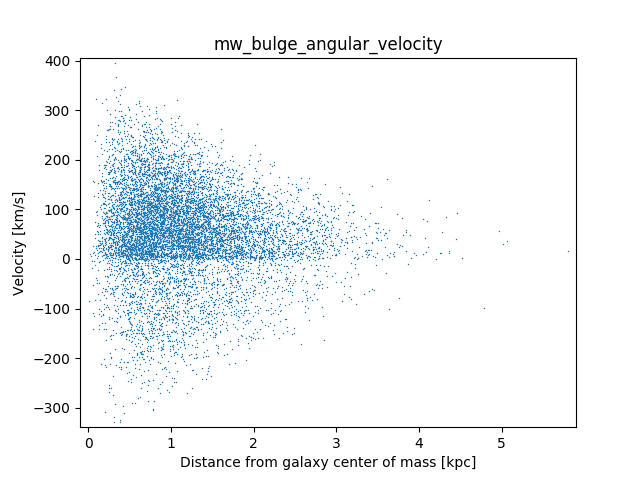
\includegraphics[width=1\textwidth]{VelocityDistr/mw_bulge_angular_velocity.png}
\end{minipage}
\begin{minipage}{0.4\textwidth}
  \centering
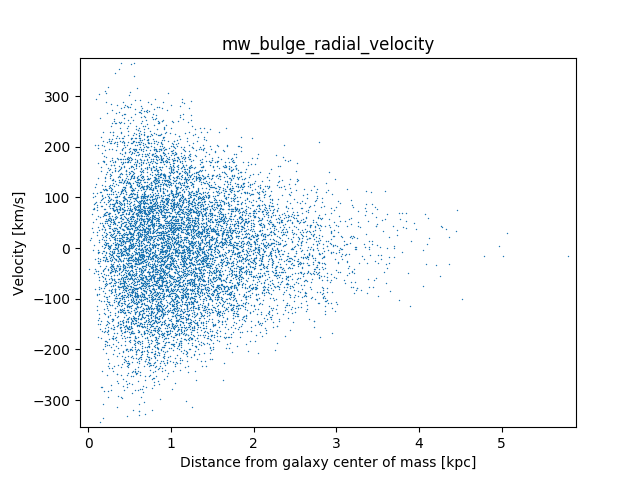
\includegraphics[width=1\textwidth]{VelocityDistr/mw_bulge_radial_velocity.png}
\end{minipage}
\begin{minipage}{0.4\textwidth}
  \centering
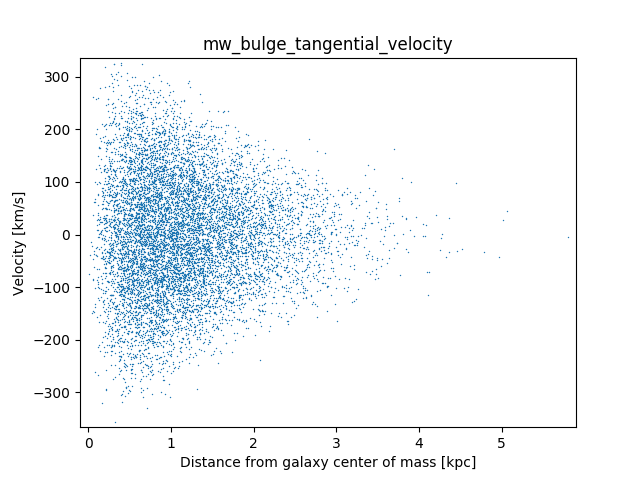
\includegraphics[width=1\textwidth]{VelocityDistr/mw_bulge_tangential_velocity.png}
\end{minipage}
\begin{minipage}{0.4\textwidth}
  \centering
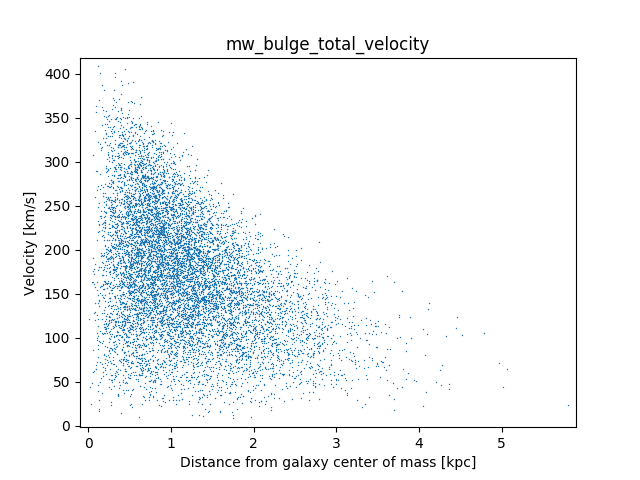
\includegraphics[width=1\textwidth]{VelocityDistr/mw_bulge_total_velocity.png}
\end{minipage}
\caption{Velocity components distribution of MW bulge particles. From left to right, top to bottom: angular velocity, radial velocity, tangential velocity and total velocity.}
\label{fig:mw-vel-distribution}
\end{figure}\par
\smallskip
In the velocity profile of the bulge particles it is clear to see that the radial and tangential velocity average out to zero, while the angular velocity has a certain rotational orientation. The variance for the velocities is also not too extreme allowing the particles to find a suitable nearby equilibrium to their position when the simulation starts. The velocity profiles for the disk and halo particles follow a similar pattern as can be seen in the appendix.\par
The rotation curve is calculated by taking the average of the total velocity magnitude at a certain distance. Doing this for the galaxies used in our simulation results in the plots as seen in figures \ref{fig:mw-rot-curve} and \ref{fig:m31-rot-curve}.\par

\begin{figure}[!h]
    \centering
    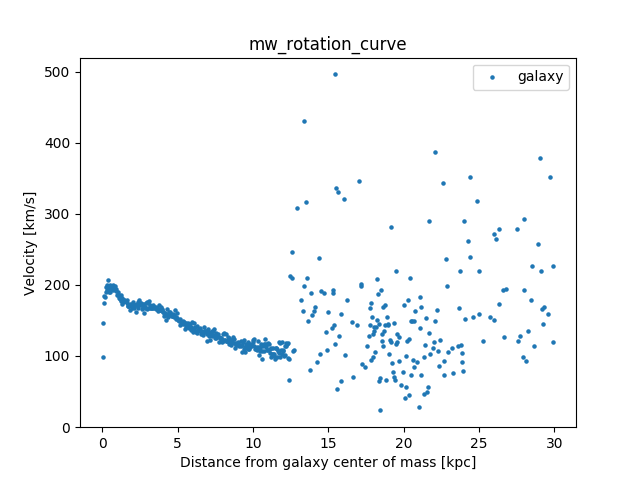
\includegraphics[width=0.6\linewidth]{VelocityDistr/mw_rotation_curve.png}
    \caption{Simulated MW rotation curve.}
    \label{fig:mw-rot-curve}
\end{figure}

\begin{figure}[!h]
    \centering
    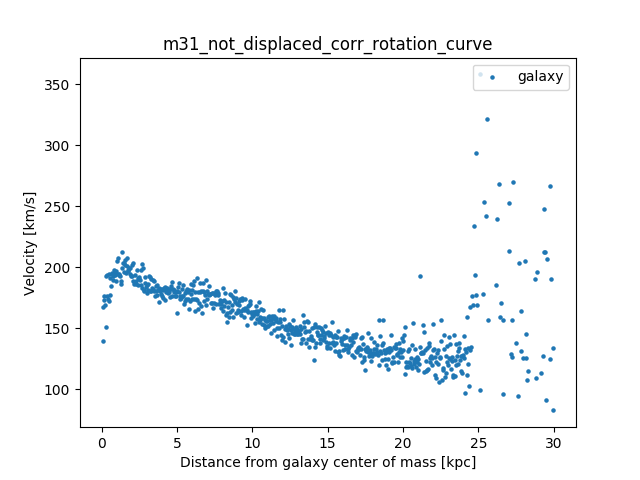
\includegraphics[width=0.6\linewidth]{VelocityDistr/m31_not_displaced_corr_rotation_curve.png}
    \caption{Simulated M31 rotation curve.}
    \label{fig:m31-rot-curve}
\end{figure}\par
\smallskip
When comparing these rotation curves with figures \ref{fig:mw-rot-curve} and \ref{fig:m31-rot-curve} we see that at closer distances it is a good fit however for longer distances the rotation of the simulation isn't as fast as in reality.\par
\smallskip
While looking at values is a great way to make sure that the initial conditions are representative of reality, this does not give the guarantee that our system will evolve how we intended it to. For this reason we ran multiple simulations to see if the particles rotate as intended and stay bounded properly. The same thing has been done including the Solar System tracker particles.\par

\begin{figure}[!h]
\centering
\begin{minipage}{0.48\textwidth}
  \centering
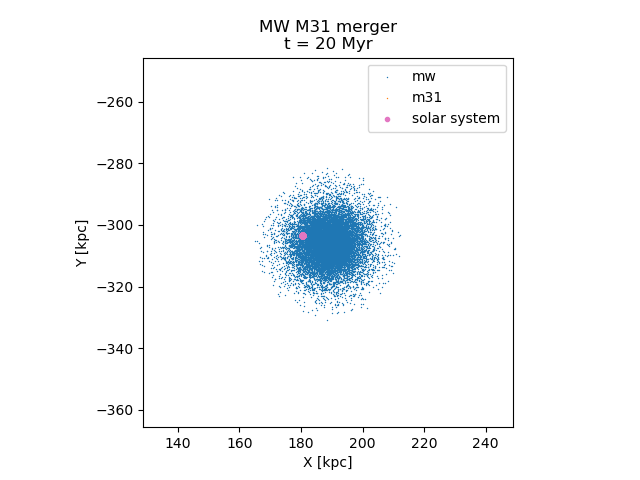
\includegraphics[width=1\textwidth]{simulations-plots/Solarevolution/mw_m31_mwzoomed_merger_0001.png}
\end{minipage}
\begin{minipage}{0.48\textwidth}
  \centering
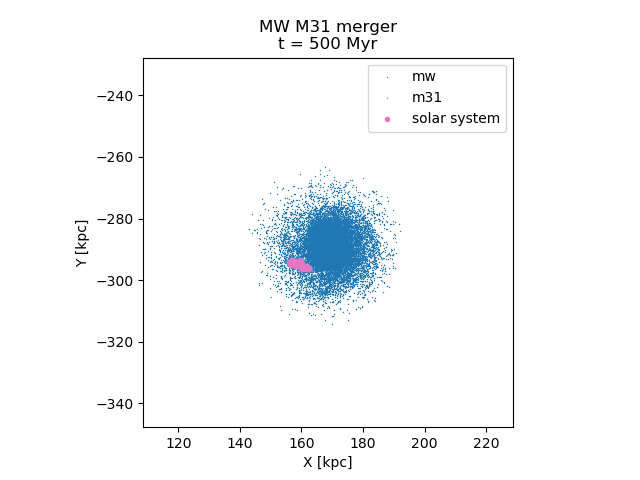
\includegraphics[width=1\textwidth]{simulations-plots/Solarevolution/mw_m31_mwzoomed_merger_0025.png}
\end{minipage}
\begin{minipage}{0.48\textwidth}
  \centering
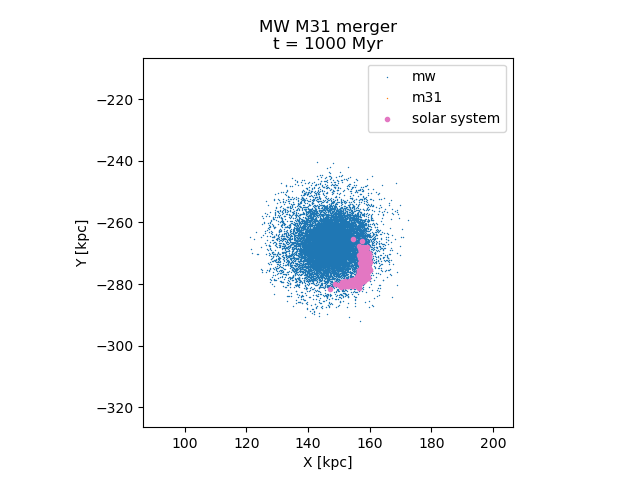
\includegraphics[width=1\textwidth]{simulations-plots/Solarevolution/mw_m31_mwzoomed_merger_0050.png}
\end{minipage}
\begin{minipage}{0.48\textwidth}
  \centering
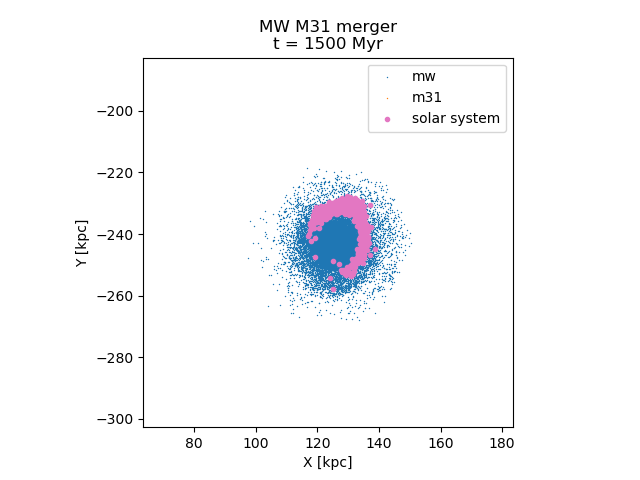
\includegraphics[width=1\textwidth]{simulations-plots/Solarevolution/mw_m31_mwzoomed_merger_0075.png}
\end{minipage}
\caption{MW particles (in blue) with Solar System trackers (in pink) at different time steps. From left to right, top to bottom: T = 20 Myr, T= 500 Myr, T= 1000 Myr and T= 1500 Myr. Snapshots of the \texttt{s72\_121220\_0003soligm} run (with \(f_r = f_t = 1\)).}
\label{fig:mw-frames}
\end{figure}
\begin{comment}
It isn't easy to see in singular frames but when playing the animation all the particles seem to be evolving as they should. 
\end{comment}
In the snapshots shown in Figure \ref{fig:mw-frames} none of the Solar System tracker particles randomly escape from the MW and they all follow a counter clockwise rotation as expected.
\subsection{Completed Runs}
\label{completed-runs}
To test a wide variety of starting velocity and quantify the impact of the IGM on the dynamics of the MW-M31 system we ran a considerable amount of simulations, presented in Tables \ref{const-radvel-runs}, \ref{const-transvel-runs} and \ref{full-runs}.\par
\smallskip
Animations of the \texttt{s72\_111220\_0010soligm}, \texttt{s72\_121220\_0003soligm} and \texttt{s72\_131220\_0001soligm} are available at \url{https://github.com/boson112358/sma-group-e-project/tree/master/final_animations}. Plots for the runs presented in Table \ref{full-runs} are also available at \url{https://github.com/boson112358/sma-group-e-project/tree/master/final_plots}.\par
\begin{table}[!h]
\centering
\begin{tabular}{@{}l|l|l|l@{}}
\toprule
Run ID               & \(f_{r}\) & \(f_{t}\) & IGM \\ \midrule
s78\_091220\_0001sol & 0.5       & 0.1       & No  \\
s78\_091220\_0002sol & 0.5       & 0.2       & No  \\
s78\_101220\_0001sol & 0.5       & 0.3       & No  \\
s78\_101220\_0002sol & 0.5       & 0.4       & No  \\
s78\_101220\_0003sol & 0.5       & 0.5       & No  \\
s72\_091220\_0001sol & 0.5       & 0.6       & No  \\
s72\_091220\_0002sol & 0.5       & 0.7       & No  \\
s72\_101220\_0001sol & 0.5       & 0.8       & No  \\
s72\_101220\_0002sol & 0.5       & 0.9       & No  \\
s72\_101220\_0003sol & 0.5       & 1         & No  \\ \bottomrule
\end{tabular}
\caption{Overview of non-IGM runs, used to test the starting transverse velocity of M31.}
\label{const-radvel-runs}
\end{table}\par

\begin{table}[!h]
\centering
\begin{tabular}{@{}l|l|l|l@{}}
\toprule
Run ID               & \(f_{r}\) & \(f_{t}\) & IGM \\ \midrule
d01\_091220\_0001sol & 0.1       & 0.5       & No  \\
d01\_101220\_0001sol & 0.2       & 0.5       & No  \\
d01\_101220\_0002sol & 0.3       & 0.5       & No  \\
d01\_101220\_0003sol & 0.4       & 0.5       & No  \\
d01\_091220\_0002sol & 0.6       & 0.5       & No  \\
d01\_101220\_0004sol & 0.7       & 0.5       & No  \\
d01\_101220\_0005sol & 0.8       & 0.5       & No  \\
d01\_101220\_0006sol & 0.9       & 0.5       & No  \\
d01\_101220\_0007sol & 1         & 0.5       & No  \\ \bottomrule
\end{tabular}
\caption{Overview of non-IGM runs, used to test the starting radial velocity of M31.}
\label{const-transvel-runs}
\end{table}
\newpage

\begin{table}[!h]
\centering
\begin{tabular}{@{}l|l|l|l@{}}
\toprule
Run ID                  & \(f_{r}\) & \(f_{t}\) & IGM \\ \midrule
s72\_121220\_0001soligm & 1         & 0.5       & Yes \\
s72\_111220\_0010soligm & 1         & 0.6       & Yes \\
s72\_121220\_0005soligm & 1         & 0.7       & Yes \\
s72\_121220\_0004soligm & 1         & 0.8       & Yes \\
s72\_131220\_0001soligm & 1         & 0.9       & Yes \\
s72\_121220\_0003soligm & 1         & 1         & Yes \\
s72\_131220\_0002soligm & 1         & 1.1       & Yes \\
s72\_131220\_0003soligm & 1         & 1.2       & Yes \\
s72\_131220\_0004sol    & 1         & 0.8       & No  \\
s72\_131220\_0005sol    & 1         & 0.9       & No  \\
s72\_121220\_0002sol    & 1         & 1         & No  \\ \bottomrule
\end{tabular}
\caption{Overview of IGM runs and non-IGM runs, used for later comparison.}
\label{full-runs}
\end{table}
\smallskip

\subsection{Phases of the Merger}\par
\begin{figure}[!h]
    \centering
    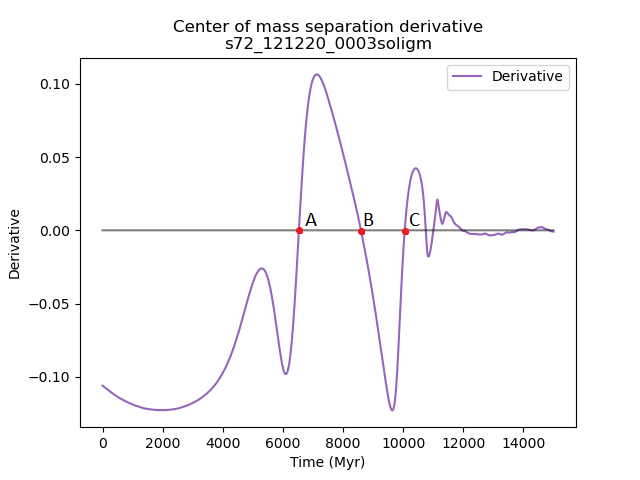
\includegraphics[width=0.8\textwidth]{separation/s72_121220_0003soligm_separation_derivative_with_points.png}
    \caption{First derivative of the centre of mass separation of the \texttt{s72\_121220\_0003soligm} run (with \(f_r = f_t = 1\)).}
    \label{fig:sep-derivative}
\end{figure}\par
Before we analyse the results, it is necessary to define the different phases of the merger. In order to do so is useful to analyse the plot of the first derivative of the galaxy centre of mass separation, shown in Figure \ref{fig:sep-derivative}. We define the first encounter, or collision (point A), as the time of the first local minimum of the separation. For different runs, we can draw out a relation between this time and different initial dynamical conditions of the system. The following phase corresponds to the time of the subsequent the local maximum of the separation (point B). The last phase we identify starts at the time of the last bump of the separation (point C), in this phase the actual merger begins as the centres of mass of both galaxies stabilise their orbit around the common centre of mass.\par
\smallskip
In Figure \ref{fig:merger-frames} are shown four XY plane snapshots of a merger simulation featuring the addition of the IGM.\par
\begin{figure}[!h]
\centering
\begin{minipage}{0.48\textwidth}
  \centering
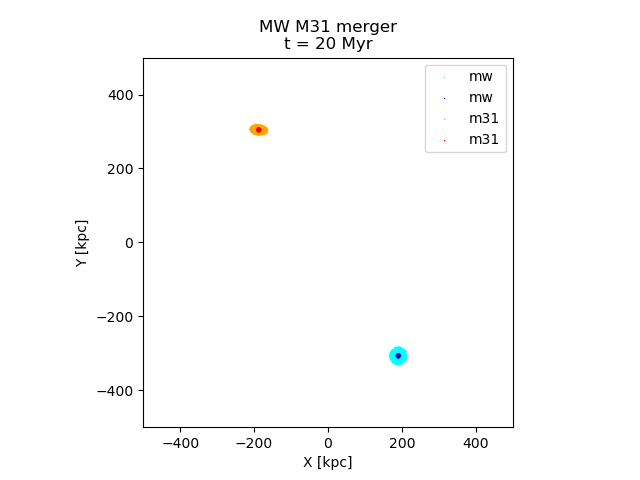
\includegraphics[width=1\textwidth]{simulations-plots/merger_snapshots/mw_m31_diskbulge_merger_0001.png}
\end{minipage}
\begin{minipage}{0.48\textwidth}
  \centering
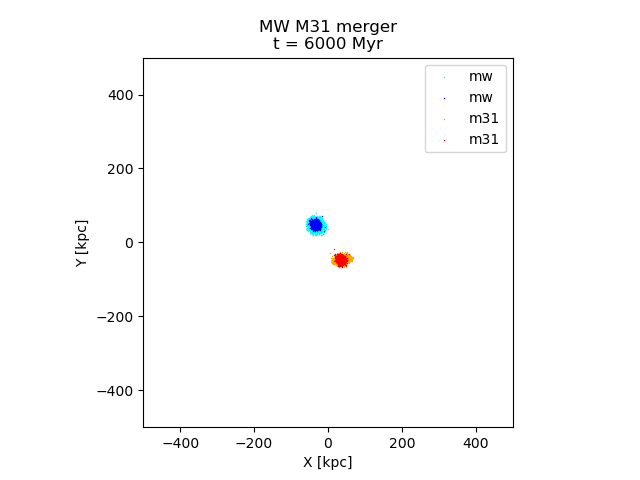
\includegraphics[width=1\textwidth]{simulations-plots/merger_snapshots/mw_m31_diskbulge_merger_0300.png}
\end{minipage}
\begin{minipage}{0.48\textwidth}
  \centering
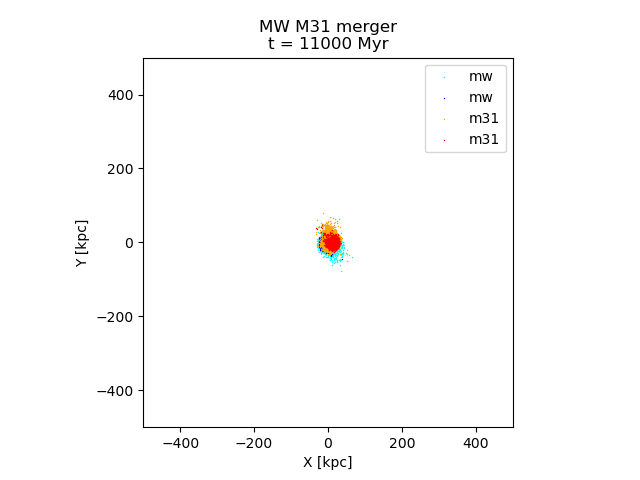
\includegraphics[width=1\textwidth]{simulations-plots/merger_snapshots/mw_m31_diskbulge_merger_0550.png}
\end{minipage}
\begin{minipage}{0.48\textwidth}
  \centering
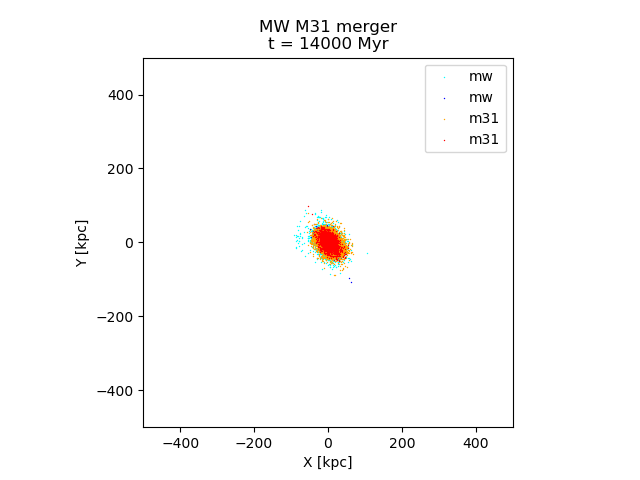
\includegraphics[width=1\textwidth]{simulations-plots/merger_snapshots/mw_m31_diskbulge_merger_0700.png}
\end{minipage}
\caption{Snapshots of the \texttt{s72\_121220\_0003soligm} run (with \(f_r = f_t = 1\)). The MW is in blue and cyan colors and M31 is in orange and red colors. From left to right, top to bottom: T = 20 Myr, T= 6000 Myr (close to the first encounter), T= 11000 Myr and T= 14000 Myr.}
\label{fig:merger-frames}
\end{figure}
\smallskip

\subsection{Non-IGM Simulation}
\label{non-igm-sim}
After analysing the stability of the models we can now present the results of our simulation runs. First we show the results of simulations without an IGM, trying different starting velocities for M31. With these simulations we can get a better idea on how these different velocities affect the fate of the merger. The main advantage of doing this in the non-IGM run is that simulations take much less time, allowing us to test a wide range of velocities.\par
\smallskip
We first look at the separation between the MW and M31 centres of mass as a function of time. By changing the radial velocity component of M31 while keeping the tangential component fixed we can see what effect this parameter has on the merger. Since there is no IGM in this simulations, the velocities we used had to be lowered by a factor \(f_t = 0.5\), in order to obtain a merger similar to the IGM simulations.\par
\begin{figure}[!h]
    \centering
    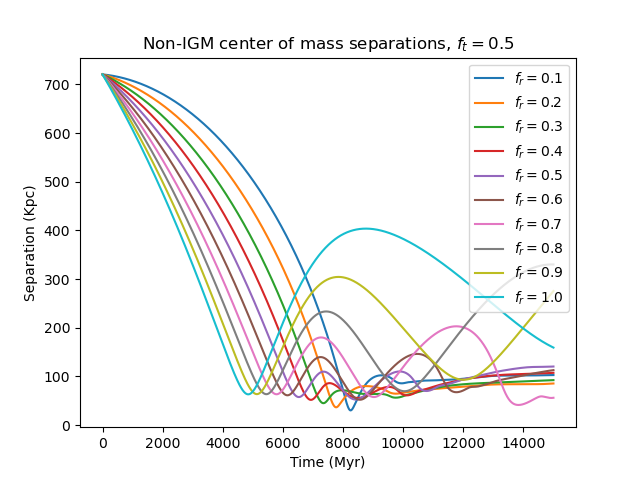
\includegraphics[width=0.9\textwidth]{separation/comparison_constant_transvel_noIGM.png}
    \caption{Separation plots between centres of mass of the galaxies with tangential velocity $v_{tan}=0.5\times 42$ km/s for M31.}
    \label{fig:No-IGM-Separation-Trans-constant}
\end{figure}
\smallskip
The separation plots can be explained by looking at the minimum and maximum points at different times. The first minimum marks the first close encounter, in these plots a higher radial velocity causes the first encounter to occur earlier.\par
\smallskip
The subsequent maximum represents the moment when the galaxies are the furthest apart after this close encounter. For $f_r=0.1$ and other low values this maximum is hard to spot, meaning that the merger finishes quickly after the first close encounter. The separation for these factors also remain constant at the end of the simulation giving us another sign that the merger has completed. For higher values like $f_r=0.9$ these bumps last for the entire duration of the simulation. This signifies that the merger was not able to complete before the end of the simulation.\par
\smallskip
Looking closely at these plots, an issue arises: as the simulations approach the end time none of the separations go to zero. This does not mean that the merger does not take place, but it could mean that the centre of mass function does not return the expected value. This might be caused by ejected particles skewing the centre of mass too harshly since there is nothing to slow them down. However when checking the animations there is a clear merger visible.\par
\smallskip
We can repeat this analysis keeping the $f_r$ factor constant while sweeping the tangential velocity factor $f_t$.\par
\begin{figure}[!h]
    \centering
    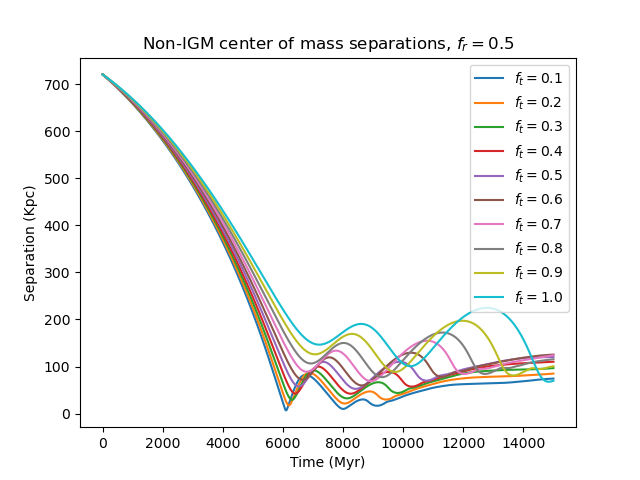
\includegraphics[width=0.9\textwidth]{separation/comparison_constant_radvel_noIGM.png}
    \caption{Separation between centre of mass of the galaxies with radial velocity $v_{rad}=0.5 \times 117$ km/s for M31.}
    \label{fig:No-IGM-Separation-Radial-constant}
\end{figure}
\smallskip
The increase of the tangential velocity delays the time of the first close encounter and it also causes it to happen at higher distances. The higher tangential factors like $f_t=1.0$ have not yet completed their merger by the end of the 15 Gyr simulation.\par
\smallskip
As happened in the previous plots (Figure \ref{fig:No-IGM-Separation-Trans-constant}), we encounter the same separation issue as it does not go to zero. But yet again the animations seem to suggest otherwise and show a clear merger for all factors up to $f_t=0.9$, for $f_t=0.9$ and higher they seem to be slightly orbiting each other while approaching .\par
\smallskip
These separation plots are used to find times on which we want to check the distribution of the Solar System tracker particles. Interesting moments to analyse on are: before the first close encounter, after the first close contact and at 15 Gyr (post-merger). Focusing on these specific times of the simulation lets us monitor how the position distribution changes as the merger event unfolds.\par
\newpage

\subsection{IGM Simulations}
\label{igm-simulations}
After the analysis of the non-IGM runs we finally include the IGM into the simulations. Due to the long computation time and because the tangential velocity of M31 $v_{rad}$ has more constraints, we focus on the transverse velocity, changing it with $f_t$ for the different simulations. Our results are shown in Figure \ref{fig:IGM-Separation}.\par
\begin{figure}[!h]
    \centering
    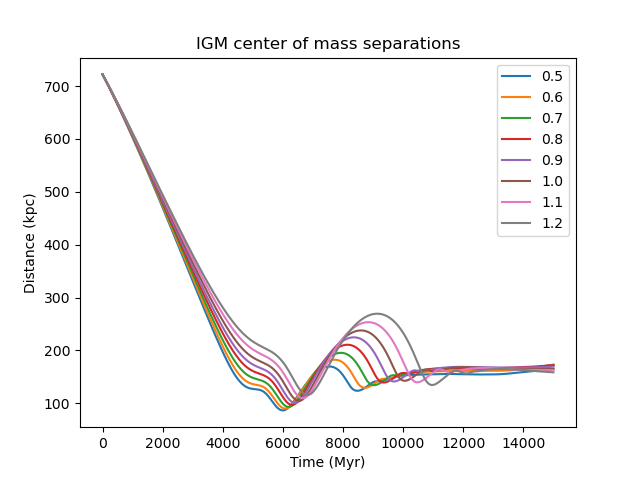
\includegraphics[width=0.9\textwidth]{separation/comparison_IGM_separation.png}
    \caption{Separation between centre of mass of the galaxies with $v_{rad}=117 km/s$ for M31.}
    \label{fig:IGM-Separation}
\end{figure}
\smallskip
This separation plots feature a slight bump around 5 Gyr before what seems to be the first close encounter, this fact is interesting because this bump is not present in the non-IGM runs. When going through the animations however it becomes clear that this bump is actually a first encounter that is quickly followed by an even closer encounter at around 6.5 Gyr. We also seem to have a similar trend for our tangential velocity as we see in our non-IGM plots. Increasing it delays the initial close encounter and causes the maximum separation afterwards to be much larger. The tangential velocity factor thus seems to be an important factor to determine how soon the merger can complete.\par
\newpage

\subsection{Effect of the IGM on the Merger}
\label{igm-effect}
\begin{figure}[!htb]
    \centering
    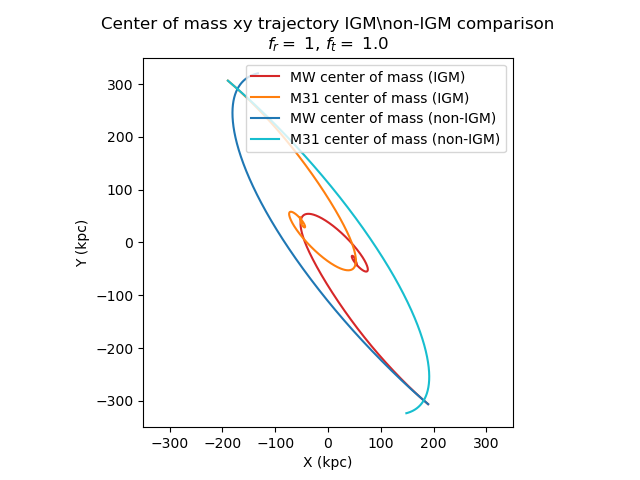
\includegraphics[width=0.9\textwidth]{_com_trajectory_IGM_comparison_tvel10.png}
    \caption{Centre of mass trajectory for IGM and non-IGM 15 Gyr run. Note how the IGM centres of mass does not seem to converge to (0,0) even though the merger occurred.}
    \label{fig:traject-comparison}
\end{figure}\par

From our simulation the influence of the IGM in the merger appears to be quite considerable. In our non-IGM runs we have to reduce either of the M31 velocity components by half in order to make the merger happen. This behaviour is more clear when we plot the centre of mass separation as a function of time (Figure \ref{fig:sep-comparison}) and their trajectory in the XY plane (Figure \ref{fig:traject-comparison}) of IGM and non-IGM runs together.\par
\newpage

\begin{figure}[!htb]
    \centering
    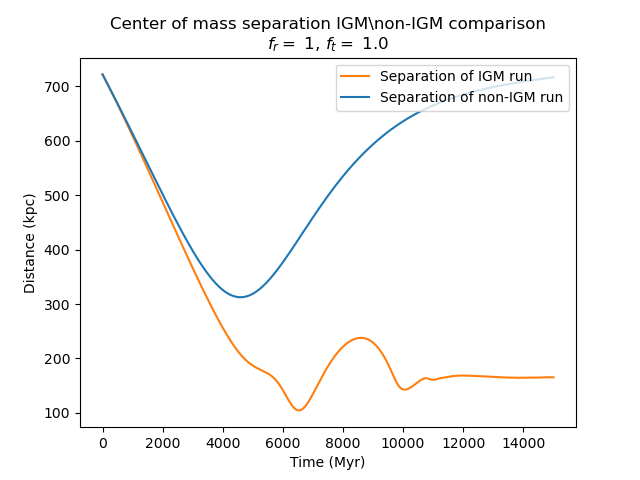
\includegraphics[width=0.9\textwidth]{separation/_separation_IGM_comparison_tvel10.png}
    \caption{Separation for IGM and non-IGM run, the IGM run seems to have a clear merger while the non-IGM only shows signs of a close encounter.}
    \label{fig:sep-comparison}
\end{figure}
\newpage

\subsection{Solar System Trackers Distribution}
\label{solar-distrib}
\begin{figure}[!h]
    \centering
    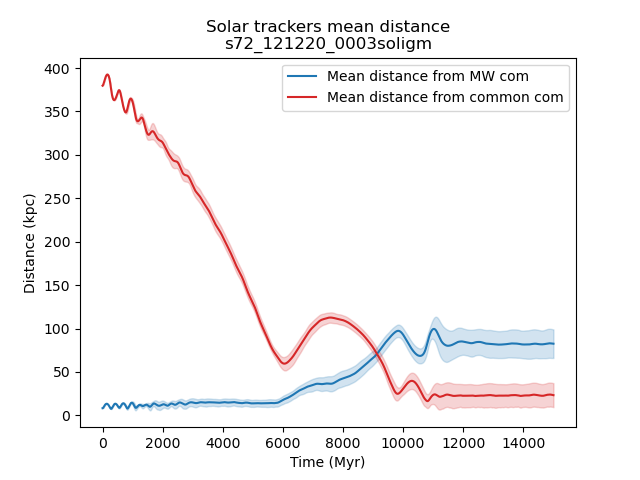
\includegraphics[width=0.9\textwidth]{separation/s72_121220_0003soligm_solar_system_mean_distance.png}
    \caption{Mean distance and variance of the Solar System trackers as a function of time. Blue: distance from the MW centre of mass. Red: distance from the MW-M31 centre of mass. From the \texttt{s72\_121220\_0003soligm} run (with \(f_r = f_t = 1\)).}
    \label{fig:solar-mean-dist}
\end{figure}
Looking at Figure \ref{fig:solar-mean-dist} we see that the distance from the MW centre of mass is a good indicator of the Solar System trackers position up to the first encounter. On the other hand the distance from the MW-M31 centre of mass is a better indicator in the final stages of the merger.\par
\newpage
\begin{figure}[!h]
    \centering
    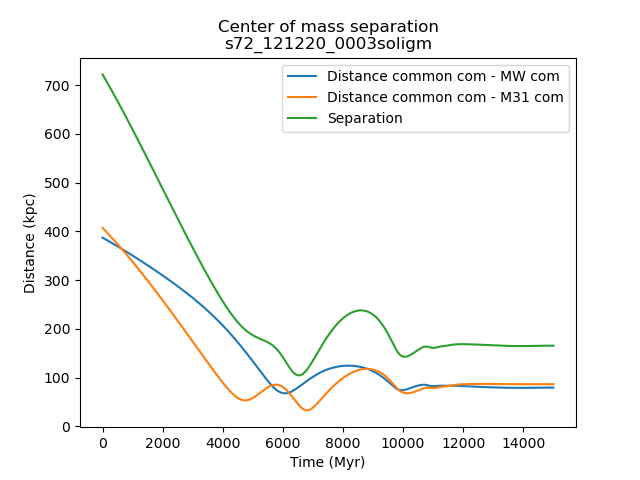
\includegraphics[width=0.9\textwidth]{separation/s72_121220_0003soligm_separation.png}
    \caption{Galaxy centre of mass separation and separation between each galaxy and MW-M31 centre of mass as a function of time. Green: galaxy separation. Blue: distance between the MW centre of mass and the MW-M31 centre of mass. Orange: distance between the M31 centre of mass and the MW-M31 centre of mass. From the \texttt{s72\_121220\_0003soligm} run (with \(f_r = f_t = 1\)).}
    \label{fig:com-separation}
\end{figure}
\smallskip
The drift of the centres of mass after the first encounter (Figure \ref{fig:com-separation}) causes issues and because of this we cannot easily calculate the distance distribution of the Solar System tracker particles in respect to the MW centre of mass. Due to this fact the distance distributions at the end of the simulations are calculated in respect to the centre of mass of the whole MW-M31 system, while the distributions before the first encounter are computed in respect to the MW centre of mass.\par
\newpage
\begin{figure}[!h]
\centering
\begin{minipage}{0.45\textwidth}
  \centering
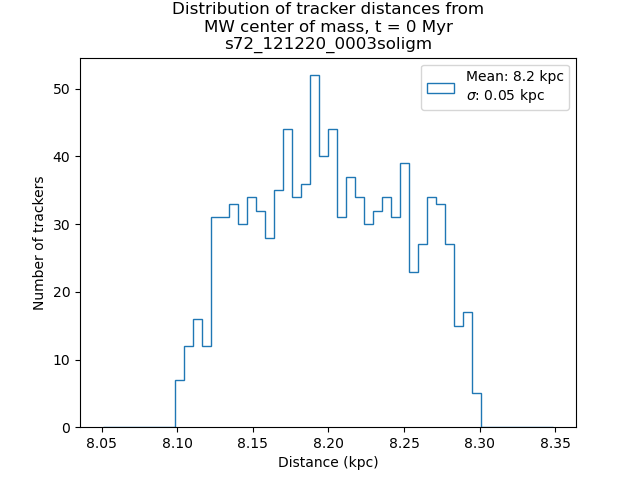
\includegraphics[width=1\textwidth]{Histogram/IGMvelfactor1/hist_mw_com_00000.png}
\end{minipage}
\begin{minipage}{0.45\textwidth}
  \centering
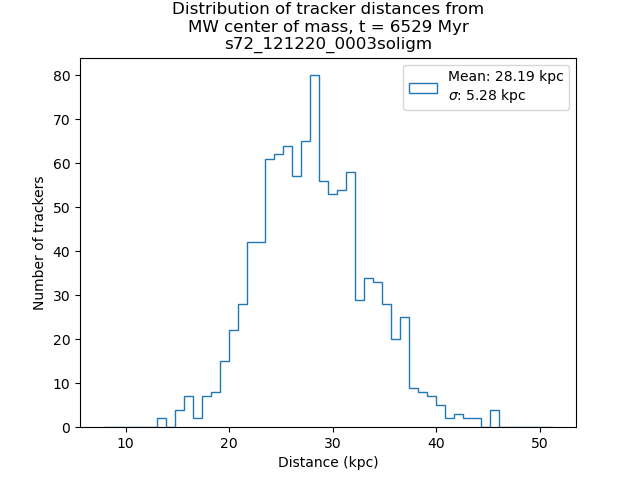
\includegraphics[width=1\textwidth]{Histogram/IGMvelfactor1/hist_mw_com_01306.png}
\end{minipage}
\begin{minipage}{0.45\textwidth}
  \centering
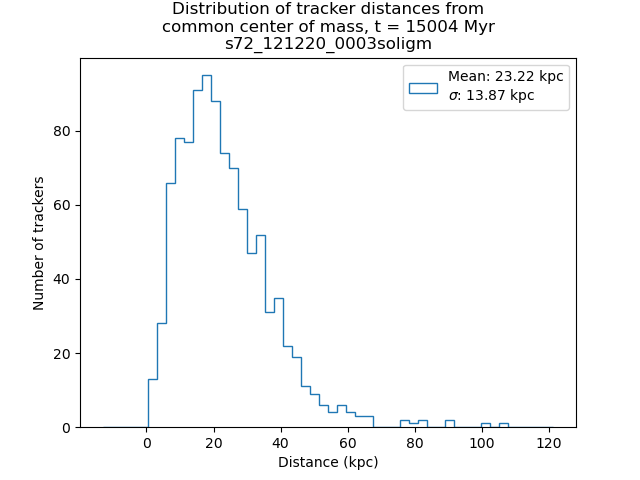
\includegraphics[width=1\textwidth]{Histogram/IGMvelfactor1/hist_common_com_-0001.png}
\end{minipage}
\caption{Statistical distribution of the 1000 Solar System tracker particles from the \texttt{s72\_121220\_0003soligm} run (with \(f_r = f_t = 1\)), at different time steps. From left to right, top to bottom: T= 0 Myr, T= 6529 Myr (first encounter), T= 15004 Myr.}
\label{fig:IGM-Hist-x}
\end{figure}
\smallskip
The first histogram gives the initial distribution of our solar system particles. The second histogram is at the time of the first encounter, due to the drift in the centre of mass however the median and variation are skewed. The final histogram is at the end of the simulation with respect to the MW-M31 centre of mass. But even though the median is more reasonable, the resulting galaxy seems to not be centred around the simulation's centre of mass.\par
\smallskip
The results of the analysis of the Solar System tracker particles distance distribution are displayed in Table \ref{tab:final-results}, where \(\bar{d}_i\) and \(\sigma_i\) are the mean distance from the MW centre of mass and its variance at the start of the simulation, \(T_e\) is the time of the first encounter and \(\bar{d}_f\) and \(\sigma_f\) are the mean distance from the MW-M31 centre of mass and its variance at the end of the simulation. All the runs feature the IGM and \(f_r = 1\). The starting Solar System tracker distribution are \(\bar{d}_i = 8.2\) kpc and \(\sigma_i = 0.005\) kpc, respectively the mean distance from the MW centre of mass and its variance.\par

\begin{table}[]
\centering
\begin{tabular}{@{}l|l|l|l|l@{}}
\toprule
Run ID                  & \(f_{t}\) & \(T_e\) (Gyr) & \(\bar{d}_f\) (kpc) & \(\sigma_f\) (kpc) \\ \midrule
s72\_121220\_0001soligm & 0.5       & 5.994         & 22.85               & 13.58              \\
s72\_111220\_0010soligm & 0.6       & 6.074         & 23.88               & 13.74              \\
s72\_121220\_0005soligm & 0.7       & 6.184         & 25.19               & 13.36              \\
s72\_121220\_0004soligm & 0.8       & 6.299         & 22.46               & 12.52              \\
s72\_131220\_0001soligm & 0.9       & 6.399         & 23.19               & 13.66              \\
s72\_121220\_0003soligm & 1         & 6.529         & 23.22               & 13.87              \\
s72\_131220\_0002soligm & 1.1       & 6.654         & 23.88               & 13.93              \\
s72\_131220\_0003soligm & 1.2       & 6.809         & 23.37               & 13.98              \\ \bottomrule
\end{tabular}
\caption{Time of the first encounter and final distance distribution of the IGM runs.}
\label{tab:final-results}
\end{table}\par
\newpage
\phantom{Just to get a new page don't mind me}
\newpage
\section{Conclusions}
\label{conclusions}
In this project we used the \texttt{GalactICs} module of the AMUSE framework to generate models of the MW and M31. Afterwards we used the \texttt{Gadget2} solver to test the stability of our models and to simulate the merger event. Inspired by the work done by \textcite{Cox_2008}, we took the IGM into consideration, as it exerts dynamical friction on galaxies. After completing the first merger simulations, we added 1000 Solar System tracker particles to the system and inferred their final position in the merged galaxy.\par
\smallskip
Due to the presence of a bug within the \texttt{GalactICs} module during the galaxy model generation, we only used the number of particles and the disk mass as parameters. Therefore, our galaxy models do not closely represent the MW and M31. Nonetheless we were able to produce meaningful results.\par
\smallskip
Then we simulated nineteen non-IGM runs, by changing the tangential and radial velocity components of M31. By plotting the separation of the centre of mass of the two galaxies for each run, we obtained our first result: the starting dynamical conditions of the MW-M31 have a great effect on the future merger evolution, particularly on the time of the first close encounter that then dictated the following evolution of the system. More precisely the greater the velocity components, the later the first encounter will take place.\par
\smallskip
Owing to the fact that the tangential velocity component of M31 is more precisely known, we ran eight IGM runs without changing the radial velocity component of M31. In this way we obtained more results: the IGM plays a major role in the merger process exerting friction on both galaxies, reducing the time of the first encounter and effectively speeding up the merger process. Furthermore the IGM also allows the merger to occur at higher velocities as opposed to a system without its presence.\par
\smallskip
Finally we monitored the evolution of the Solar System tracker particles during the merger process and plotted several histograms to show their distance distribution in various stages of the merger. Analysing these distance distribution we obtained our final results: it appears that at the end of the merger the average position of the Solar System tracker particles will be further away from the centre of the newly formed galaxy, compared to its starting radial coordinate in the MW. In addition we did not observe any ejected tracker in any stage of the merger.\par
\smallskip
This project has many possible future developments:
\begin{itemize}
    \item first of all, a fix of the \texttt{GalactICs} bug could lead to more detailed galaxy models and so to a more precise analysis of the Solar System trackers;
    \item the study of the galaxy separation could also be improved, in this report we mentioned the drift of the galaxies' centre of mass as an issue against the correct interpretation of the separation. A fix in the code could lead to more precise merger dynamic analysis;
    \item the dynamical evolution of the central supermassive black holes could also be taken into consideration in future works;
    \item in the last years the GAIA mission has provided the astrophysical community with a large quantity of data, that is leading to more precise constraints on the Local Group dynamics. For instance \textcite{van_der_Marel_2019} presents new and exciting measurements of the relative velocity not only of M31, but also for other massive members of the Local Group, such as M31 and the LMC. These galaxies are expected to play an important role in the MW-M31 merger and any future work should try to implement these elements into the simulations, to obtain a more precise merger simulation.
\end{itemize}\par
\smallskip
In conclusion we learned a lot about the future MW-M31 merger, its dynamical evolution and the effect that both the starting conditions and the IGM have on the system, but a lot of research remains to be done to finally give a precise and satisfactory answer to the question "What will be the fate of the Solar System after the merger?".



\iffalse At the time of writing this report, a viable simulation to draw conclusions from has not been produced. The main issue is due to the initial conditions of the galaxy. When using \texttt{GalactICs} with the parameters described in Section \ref{mw-m31-models}, the resulting galaxy is not stable over timescales long enough to effectively simulating the merger, as shown in Figures \ref{fig:mw-m31-merger-evolution} and \ref{fig:mw-evolution}. We believe that the reason is that our models feature larger mass and velocity compared to the expected values. Currently we do not know what is causing this discrepancy and we are currently putting all our efforts into fixing it.\par
\smallskip

\subsection{Current issues}
The first problem that we noticed was the wrong timescale for the merger event. During the first simulations the merger event started after \(\approx 500\) Myr, instead of the 5 Gyr proposed by earlier works (\textcite{Cox_2008},\textcite{van_der_Marel_2019} and \textcite{Schiavi_2019}). It turned out that the mass for our galaxies was incorrect with an order of $10^3$, namely \(1.7 \times 10^{15}\: M_{\odot}\) compared to the expected mass of \(\approx 10^{12}\: M_{\odot}\) (see \textcite{Watkins_2019}). For now this is resolved by multiplying the total galaxy mass by a  $10^{-3}$ factor. However this is just a temporary solution, this issue should be properly solved by changing the dimensionality parameter of the halo of the galaxy. Within the \texttt{GalactICs} module the extension of the halo dictates the final mass of the total galaxy. In the plots in Section \ref{resutls} we can see that the halo radius is 6000 kpc, which is obviously too wide. If we eventually manage to shrink the galaxy halo we will be able to solve the mass discrepancy issue.\par
\smallskip
The second issue is the starting velocity of the galaxy particles, that gives rise to an extreme instability of the models. After a few Myr into the merger simulation, both galaxies feature a steady expansion of their radii, caused by the motion of their particles, outwards from their centre. After performing an analysis of the models, as presented in Section \ref{model-analysis} and shown in Section \ref{resutls}, we gained some insight on this issue: the velocity of the particles is too large to keep the particles bound to each galaxy. This huge range of particle velocities needs to be reduced to make sure that our galaxy models are stable on timescales comparable to the time span of the merger event (\(\gtrsim\) 5 Gyr).\par
\smallskip
A first correction was attempted by multiplying the cartesian velocity of each particle with a factor to reduce its magnitude, as previously stated in Section \ref{resutls}. While this approach initially works in reducing the total velocity to the right value $\pm 200\frac{km}{s}$, it does not help to keep the galaxies stable on large timescales. We consequently used smaller factors (down to 0.05) to further reduce the velocity, however this approach only led to the collapse of the galaxies.\par
\smallskip
These are our main issues at the moment and as soon as we can solve them, we are ready to run our simulation and get results. Our current hypothesis is that the \texttt{central\_radial\_vel\_dispersion} parameter of the \texttt{GalactICs} module should have an effect on the variance of the velocities, however it is only defined for the disk particles. We are going to further analyse the effect of this parameter on the galaxies, hoping to obtain a meaningful result.\par
\smallskip
In the case that this method does not work, \texttt{get\_scale\_velocity} and other scale parameters might have to be changed to see which one has an effect on the variance. Another theory is that our issues rise from a combined effect of wrong total mass and of small value of the halo cut-off radius. Fixing the cut-off radius and consequently the total mass might be enough to solve our velocity dispersion issues.\par
\smallskip
The worst case scenario would happen if we are not able to get the \texttt{GalactICs} initialisation working properly. In this case we will write our own code to make a simplified galaxy model. We are fully aware that this is the least preferred option as it will take a long time to properly implement.\par

\subsection{Future developments}
Our current main priority is to fix the galaxy models, focusing on reproducing the observed rotation curves in order to stabilize both galaxies. After this fundamental step, we will run several merger simulations, aiming to produce meaningful animations and plots of this event between the MW and M31. Our goals are to reproduce typical merger features, such as tidal tails, and to track the dynamical evolution of the Solar System. Once this has been completed it will be possible to test different transverse velocity of M31 to check the dependence of the merger on this parameter. We will keep tracking the Solar System during the process and determine its statistical likelihood to remain bound to the newly formed galaxy after the merger and final position.\par
\smallskip
After evolving the model without taking the IGM into account, we will attempt to add a homogeneous IGM, which is initially a constant density cube of 1.5 Mpc on a side composed of both dark matter and gas (see \textcite{Cox_2008}). Then we need to determine the initial conditions of IGM, such as the number of IGM particles, the density of IGM and the internal energy of the gas. In addition to the merger analysis, we will also focus on how the galaxy affects the IGM particles during the merging process.\par
\smallskip
If there will be enough time, the last thing we aim to do is adding the a SMBHs to both galaxies and monitor their motion. Similarly, we will try different transverse velocity of M31 to obtain the separation between the two SMBHs as function of time for the different values.\par
\fi
\newpage
\setlength\bibitemsep{0.5\baselineskip}
\printbibliography[heading=bibintoc,title={References}]


\appendix
\section{Velocity Components}
\label{Appendix}
\begin{figure}[!h]
\centering
\begin{minipage}{0.45\textwidth}
  \centering
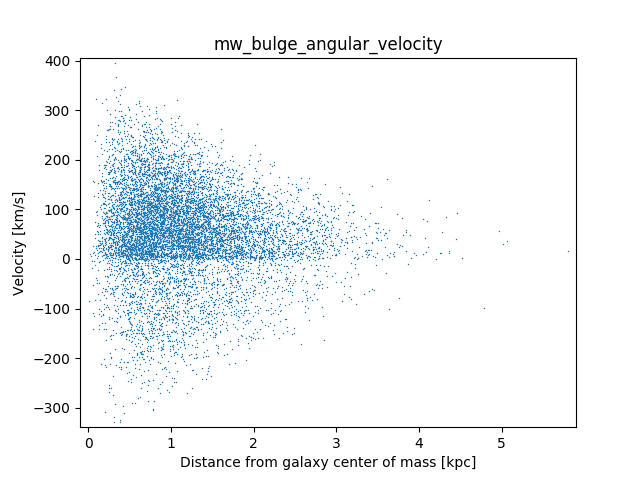
\includegraphics[width=1\textwidth]{VelocityDistr/mw_bulge_angular_velocity.png}
\end{minipage}
\begin{minipage}{0.45\textwidth}
  \centering
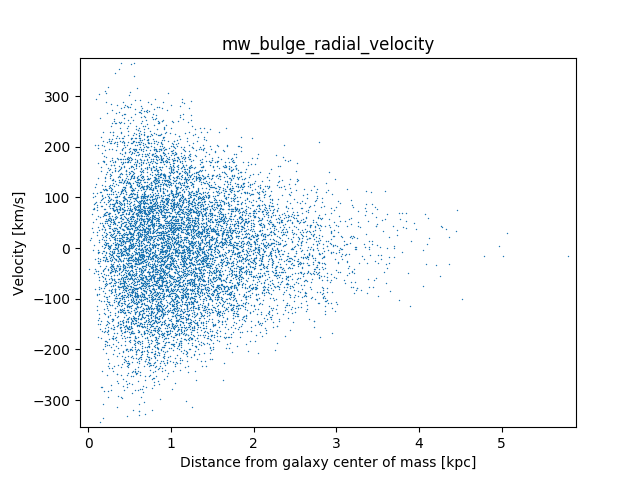
\includegraphics[width=1\textwidth]{VelocityDistr/mw_bulge_radial_velocity.png}
\end{minipage}
\begin{minipage}{0.45\textwidth}
  \centering
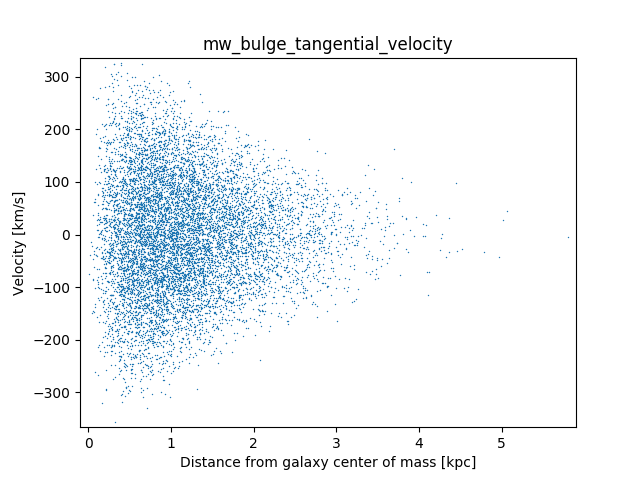
\includegraphics[width=1\textwidth]{VelocityDistr/mw_bulge_tangential_velocity.png}
\end{minipage}
\begin{minipage}{0.45\textwidth}
  \centering
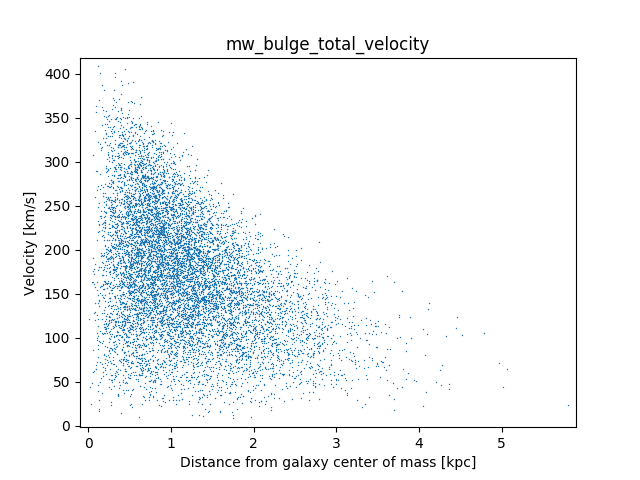
\includegraphics[width=1\textwidth]{VelocityDistr/mw_bulge_total_velocity.png}
\end{minipage}
\caption{Velocity components distribution of MW bulge particles, note that the velocity has been multiplied by a 0.15 factor. From left to right, top to bottom: angular velocity, radial velocity, tangential velocity and total velocity.}
\label{fig:bulge-vel}
\end{figure}

\begin{figure}
\centering
\begin{minipage}{0.45\textwidth}
  \centering
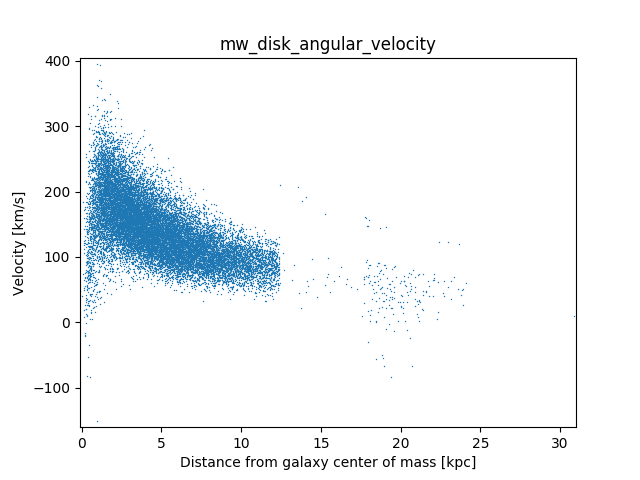
\includegraphics[width=1\textwidth]{VelocityDistr/mw_disk_angular_velocity.png}
\end{minipage}
\begin{minipage}{0.45\textwidth}
  \centering
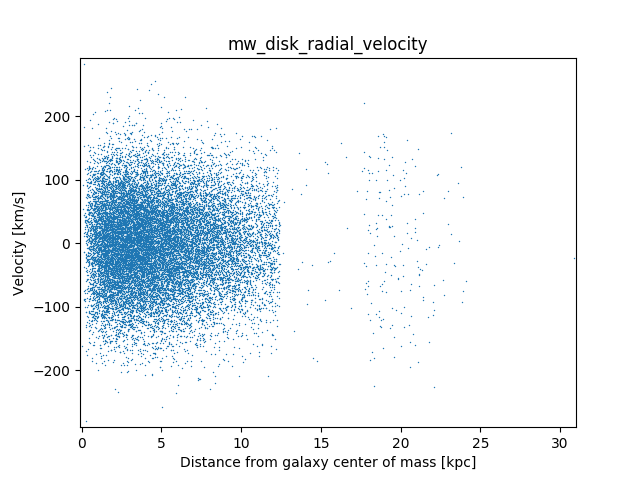
\includegraphics[width=1\textwidth]{VelocityDistr/mw_disk_radial_velocity.png}
\end{minipage}
\begin{minipage}{0.45\textwidth}
  \centering
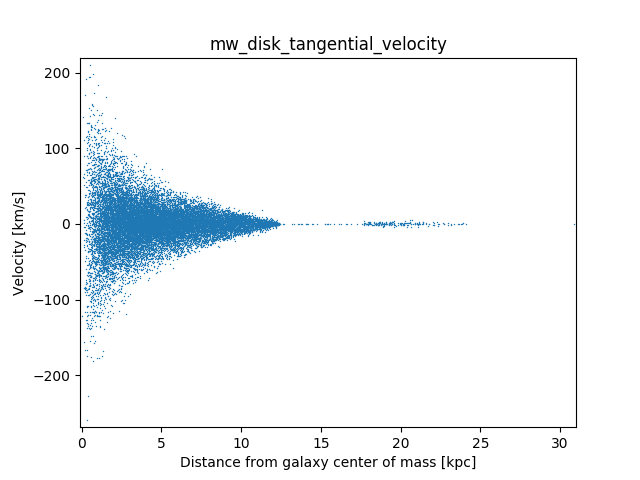
\includegraphics[width=1\textwidth]{VelocityDistr/mw_disk_tangential_velocity.png}
\end{minipage}
\begin{minipage}{0.45\textwidth}
  \centering
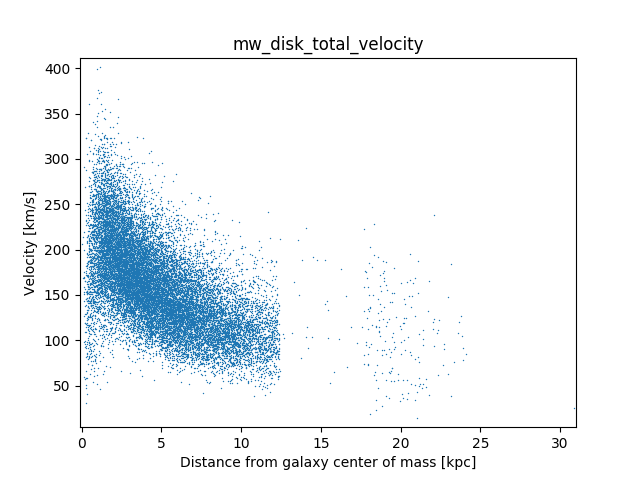
\includegraphics[width=1\textwidth]{VelocityDistr/mw_disk_total_velocity.png}
\end{minipage}
\caption{Velocity components distribution of MW disk particles, note that the velocity has been multiplied by a 0.15 factor. From left to right, top to bottom: angular velocity, radial velocity, tangential velocity and total velocity.}
\label{fig:disk-vel}
\end{figure}

\begin{figure}
\centering
\begin{minipage}{0.45\textwidth}
  \centering
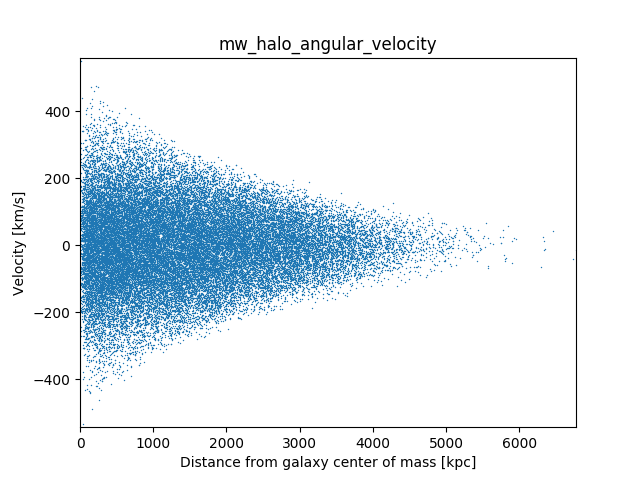
\includegraphics[width=1\textwidth]{VelocityDistr/mw_halo_angular_velocity.png}
\end{minipage}
\begin{minipage}{0.45\textwidth}
  \centering
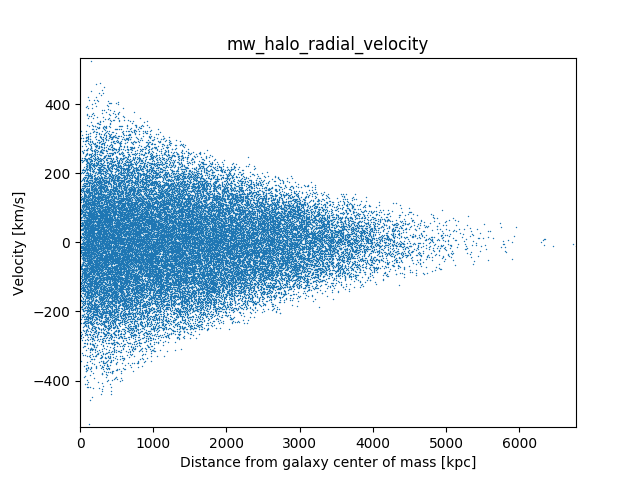
\includegraphics[width=1\textwidth]{VelocityDistr/mw_halo_radial_velocity.png}
\end{minipage}
\begin{minipage}{0.45\textwidth}
  \centering
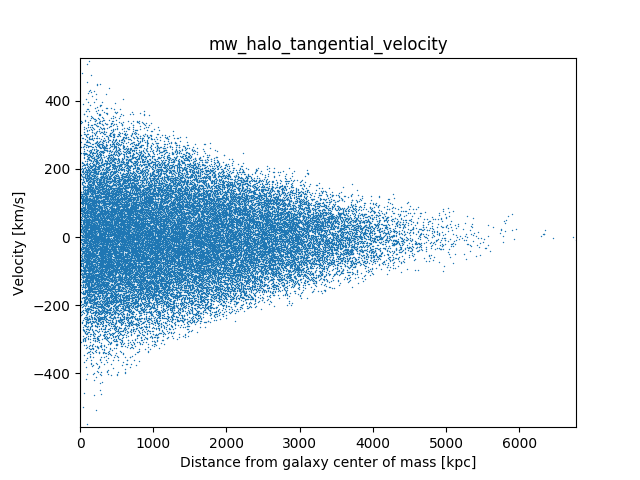
\includegraphics[width=1\textwidth]{VelocityDistr/mw_halo_tangential_velocity.png}
\end{minipage}
\begin{minipage}{0.45\textwidth}
  \centering
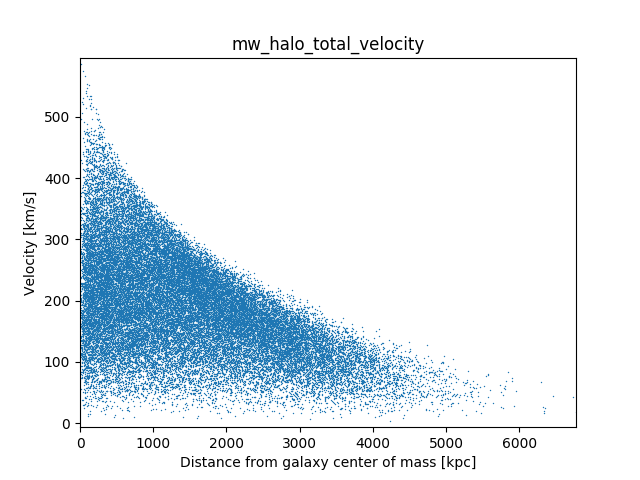
\includegraphics[width=1\textwidth]{VelocityDistr/mw_halo_total_velocity.png}
\end{minipage}
\caption{Velocity components distribution of MW halo particles, note that the velocity has been multiplied by a 0.15 factor. From left to right, top to bottom: angular velocity, radial velocity, tangential velocity and total velocity.}
\label{fig:halo-vel}
\end{figure}
\end{document}